%%%%%%%%%%%%%%%%%%%%%%%%%%%%%%%%%%%%%%%%%%%%%%%%%%%%%%%%%%%%%%%%%%%%%%%%
\chapter{Pre-training Strategy for Improving Clinical Skin Lesion Image Classifier's Performance Using Dermoscopic Images}\label{chap:Pretraining}\chaptermark{Pre-training Strategy}
%%%%%%%%%%%%%%%%%%%%%%%%%%%%%%%%%%%%%%%%%%%%%%%%%%%%%%%%%%%%%%%%%%%%%%%%

\begin{center}
	\begin{minipage}{0.8\textwidth}
		\begin{small}
			This chapter addresses research question \ref{question1}, presents our pre-training strategy for improving clinical skin lesion image classification performance of ImageNet pre-trained convolutional neural networks by utilizing additional pre-training with dermoscopic images. It also contains benchmarking of state-of-the-art convolutional architectures for Lyme disease image classification. Contents from this chapter have been used in the following article:
			\begin{itemize}
				\item \fullcite{Hossain2022}
			\end{itemize}  
		\end{small}
	\end{minipage}
	\vspace{0.5cm}
\end{center}

\minitoc

%%%%%%%%%%%%%%%%%%%%%%%%%%%%%%%%%%%%%%%%%%%%%%%%%%%%%%%%%%%%%%%%%%%%%%%%
\section{Introduction}
%%%%%%%%%%%%%%%%%%%%%%%%%%%%%%%%%%%%%%%%%%%%%%%%%%%%%%%%%%%%%%%%%%%%%%%%
%\begin{table}
%	\caption{A stunning table}
%	\label{tbl:excel-table}
%	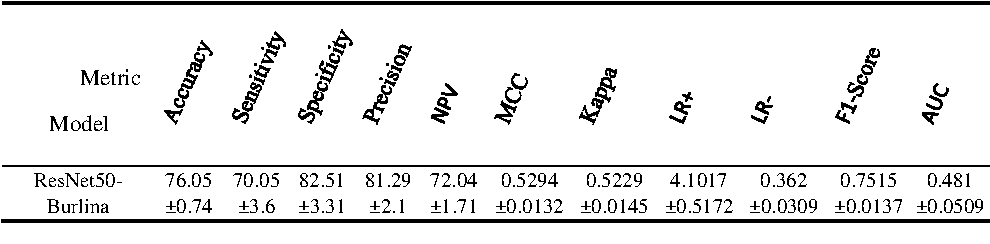
\includegraphics[width=\linewidth]{images/pretraining/ResNet50Table-cropped.pdf}
%\end{table}
Our pre-training strategy involves fine-tuning some layers from the end of an ImageNet pre-trained convolutional neural network (CNN) architecture using a dermoscopic dataset before training the model on a clinical skin lesion dataset. Our intuition behind the approach is the fact that even though the image modality of dermoscopic and clinical skin lesion images are different, pre-training some layers from the end of the model with dermoscopic images should provide a good feature representation for starting training with clinical skin lesion images. As the layers at the end of a CNN architecture respond to task-specific complex patterns, there should be a similarity between the skin lesion patterns of clinical and dermoscopic skin lesion images. We tested our strategy using dermoscopic images of skin cancer from HAM10000 dataset \cite{Tschandl2018} and clinical skin lesion images related to erythema migrans (EM).


As there is no expert-verified publicly available Lyme dataset of EM images, first, we created a dataset consisting of 866 images of confirmed EM lesions. Images collected from the internet and Clermont-Ferrand University Hospital Center (CF-CHU) of France were carefully labeled into two classes: EM and Confuser, by expert dermatologists and infectiologists from CF-CHU. CF-CHU collected the images from several hospitals in France.

Lightweight CNN-based mobile applications can help people with an initial self-assessment of EM and refer them to expert dermatologist for further diagnosis. Also, resource-intensive CNN-based computer applications can assist non-expert practitioners in identifying EM. In this chapter, besides testing our pre-training strategy, we also studied the performance of state-of-the-art CNNs for diagnosing Lyme disease from EM images and to find out the best architecture based on different criteria. We benchmarked twenty-five well-known CNNs on the prepared dataset in terms of several predictive performance metrics, computational complexity metrics, and statistical significance tests. Alongside our proposed pre-training strategy other best practices for training CNNs on limited data were used. For visualizing the regions of the input image that are significant for predictions from the CNN models we used gradient-weighted class activation mapping (Grad-CAM) \cite{Selvaraju2020}. We provided guidelines for model selection based on predictive performance and computational complexity. Moreover, we made all the trained models publicly available which can be used for transfer learning and building pre-scanners for Lyme disease. Figure \ref{fig:visualization-benchmark} presents the graphical overview of the study performed in this chapter.

The rest of the chapter is structured as follows: Section \ref{sec:matandmeth} contains the proposed pre-training strategy, dataset description, a brief overview of CNN architectures, and performance measures; Section \ref{sec:exp_result_pretrain} presents experimental studies, results, discussion, and recommendations for model selections; finally, Section \ref{sec:concluion_pretrain} presents concluding remarks.
%%%%%%%%%%%%%%%TO-DO%%%%%%%%%%%%%%%%%%%%%
\begin{figure}[htb!]
	\centering
	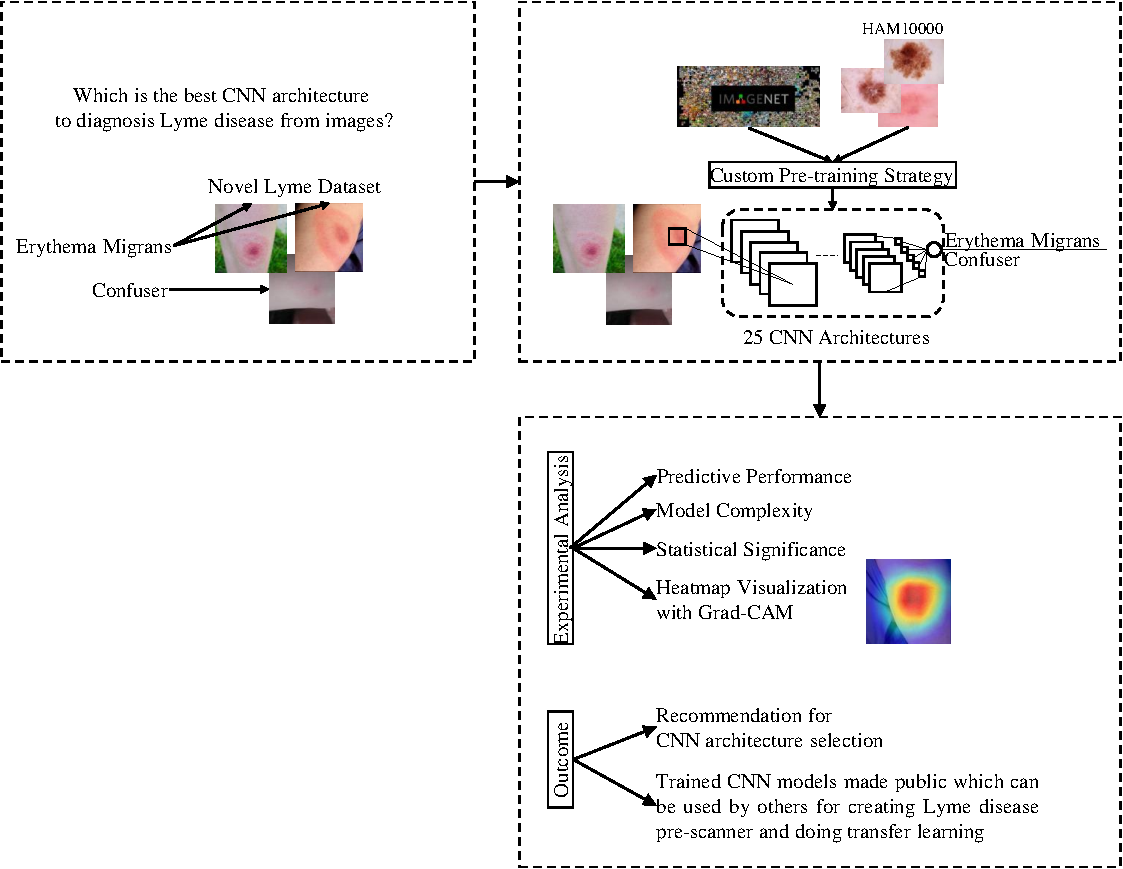
\includegraphics[width=\textwidth,keepaspectratio]{images/pretraining/Visualization-cropped.pdf}
	\caption{Graphical overview of the study on the effectiveness of CNNs utilizing custom pre-training strategy for the diagnosis of Lyme disease from images.}
	\label{fig:visualization-benchmark}
\end{figure}
%%%%%%%%%%%%%%%%%%%%%%%%%%%%%%%%%%%%%%%%%%%%%%%%%%%%%%%%%%%%%%%%%%%%%%%%
\section{Materials and Methods}\label{sec:matandmeth}
%%%%%%%%%%%%%%%%%%%%%%%%%%%%%%%%%%%%%%%%%%%%%%%%%%%%%%%%%%%%%%%%%%%%%%%%
The following subsections describe the pre-training strategy used in this study, the data organization, a short overview of the considered CNN architectures, performance measures, and heatmap visualization method.
%%%%%%%%%%%%%%%%%%%%%%%%%%%%%%%%%%%%%%%%%%%%%%%%%%%%%%%%%%%%%%%%%%%%%%%%
\subsection{Pre-training Strategy}\label{sec:pretraining-strag}
%%%%%%%%%%%%%%%%%%%%%%%%%%%%%%%%%%%%%%%%%%%%%%%%%%%%%%%%%%%%%%%%%%%%%%%%
\SetAlFnt{\small}
%\SetAlCapFnt{\t}
%\SetAlCapNameFnt{\large}
\SetKwProg{Fn}{Function}{}{}
\begin{algorithm}[htb!]
	\DontPrintSemicolon
	\SetKwFunction{findLayersToUnfreeze}{findLayersToUnfreeze}
	\SetKwInOut{KwIn}{Data}
	\SetKwInOut{KwOut}{Output}
	
	\KwIn{\newline ImageNet pre-trained CNN model without classfication head: $M_{I}$\newline
		Total layers in $M_{I}$: $N_{L}$\newline
		Dermoscopic image classification task: $\mathcal{T}_{S}$\newline
		Dermoscopic image dataset: $D_{S}$\newline
		Clinical skin lesion image classification task: $\mathcal{T}_{T}$\newline
		Clinical skin lesion image dataset: $D_{T}$\newline
	}
	
	\KwOut{\newline CNN model optimized for $\mathcal{T}_{T}: M_{T}$}
	
	\Begin{
		$M_{I} \gets$ freeze all the layers of $M_{I}$\tcp*[f]{make layers non-trainable}\;
		$U_{L} \gets$ findLayersToUnfreeze($M_{I}$, $N_{L}$, $\mathcal{T}_{T}$, $D_{T}$)\;
		$M_{S} \gets$ add classifier head to $M_{I}$ for $\mathcal{T}_{S}$\;
		\tcc{models are trained and validated using training and validation subsets of the respective dataset}
		$M_{S} \gets$ train $M_{S}$ and fine-tune after unfreezing layers $N_{L}-U_{L}+1$ to $N_{L}$ on $D_{S}$\;
		$M_{S} \gets$ freeze all the layers of $M_{S}$\;
		$M_{T} \gets$ from $M_{S}$ remove classifier head for $\mathcal{T}_{S}$ and add classifier head for $\mathcal{T}_{T}$\;
		$M_{T} \gets$ train $M_{T}$ and fine-tune after unfreezing layers $N_{L}-U_{L}+1$ to $N_{L}$ on $D_{T}$\;
		\KwRet{$M_{T}$}
	}	
	
	\Fn{findLayersToUnfreeze ($M$, $N$, $\mathcal{T}$, $D$)}{
		$M_{T} \gets$ add classifier head to $M$ for $\mathcal{T}$\;
		$\tilde{M}_{T} \gets$ train $M_{\mathcal{T}}$ using training data from $D$\;
		$U \gets 0$ \tcp*[f]{number of layers to unfreeze}\;
		$max \gets 0$ \tcp*[f]{tracks best model accuracy on validation data}\;
		\For{$i \gets 1$ \textbf{to} $N$} {
			$M_{T} \gets$ unfreeze layers $N-i+1$ to $N$ of  $M_{T}$\tcp*[f]{make  layers trainable}\; 
			$M_{T} \gets$ fine-tune $M_{T}$ using training data from $D$\;
			$temp \gets$ measure accuracy of $M_{T}$ on validation data from $D$\;
			\If{$temp > max$} {
				$max \gets temp$\;
				$U \gets i$\;
			}   
			$M_{T} \gets \tilde{M}_{T}$\;
		}
		
		\KwRet{$U$}
	}
	
	\caption{Dermoscopic pre-training for clinical lesion image classification}
	\label{algo:pretraining}	
\end{algorithm}
Algorithm \ref{algo:pretraining} shows the steps of our pre-training strategy. We start with an ImageNet pre-trained CNN model $M_{I}$ without the original ImageNet classification head. The total layers in $M_{I}$ is $N_{L}$. The source dermoscopic image classification task and dataset are $\mathcal{T}_{S}$, and $D_{S}$, respectively. The target clinical skin lesion image classification task and dataset are $\mathcal{T}_{T}$, and $D_{T}$, respectively. Initially, all the layers of $M_{I}$ are frozen to make sure the parameters are not updated during training. Then, we find out the best number of layers $U_{L}$ of $M_{I}$ to unfreeze and fine-tune for  $\mathcal{T}_{T}$ using the function \textit{findLayersToUnfreeze}. The function first adds a classification head to $M_{I}$ for $\mathcal{T}_{T}$ and trains the model using $D_{T}$. Then, the function trains the model by making different frozen layers trainable and the number of unfrozen layers giving the best validation accuracy is returned. $M_{I}$ is again pre-trained and fine-tuned using $D_{S}$ based on $U_{L}$. For that purpose, we add classification head to  $M_{I}$  for $\mathcal{T}_{S}$ resulting in a model called $M_{S}$. $M_{S}$ is trained and fine-tuned after unfreezing layers $N_{L}-U_{L}+1$ to $N_{L}$ using $D_{S}$. Then all the layers of $M_{S}$ are made non-trainable again. After pre-training and fine-tuning the unfrozen part of the model for $\mathcal{T}_{S}$, the learned feature representation is reused for $\mathcal{T}_{T}$. We remove the classifier head for $\mathcal{T}_{S}$ from $M_{S}$ and add the classifier head for $\mathcal{T}_{T}$ resulting in a model called $M_{T}$. Finally, $M_{T}$ is trained and fine-tuned after unfreezing layers $N_{L}-U_{L}+1$ to $N_{L}$ using $D_{S}$. We tested the proposed pre-training strategy on EM classification task as shown in Figure \ref{fig:pre-training}. The source dermoscopic image classification task $\mathcal{T}_{S}$ and dataset $D_{S}$ are skin cancer classification and HAM10000 dataset respectively. The target clinical skin lesion image classification task $\mathcal{T}_{T}$ and dataset $D_{T}$ are EM classification and Lyme dataset respectively. Our EM classification head consists of global average pooling (GAP) layer \cite{Lin2014}, dropout layer \cite{Srivastava2014}, and a fully connected layer with sigmoid activation for binary classification. Each channel in the feature map is averaged over the whole spatial extent by GAP, and the end result is a single value for each channel that summarizes the spatial information of the feature map. Dropout is a deep learning regularization method used to avoid overfitting. During each training iteration, a portion of the units or neurons in a layer are randomly dropped out (i.e., set to zero) by the dropout layer. As it can no longer rely on any one neuron, this forces the network to learn more reliable and generalizable features.
\begin{figure}[htb!]
	\centering
	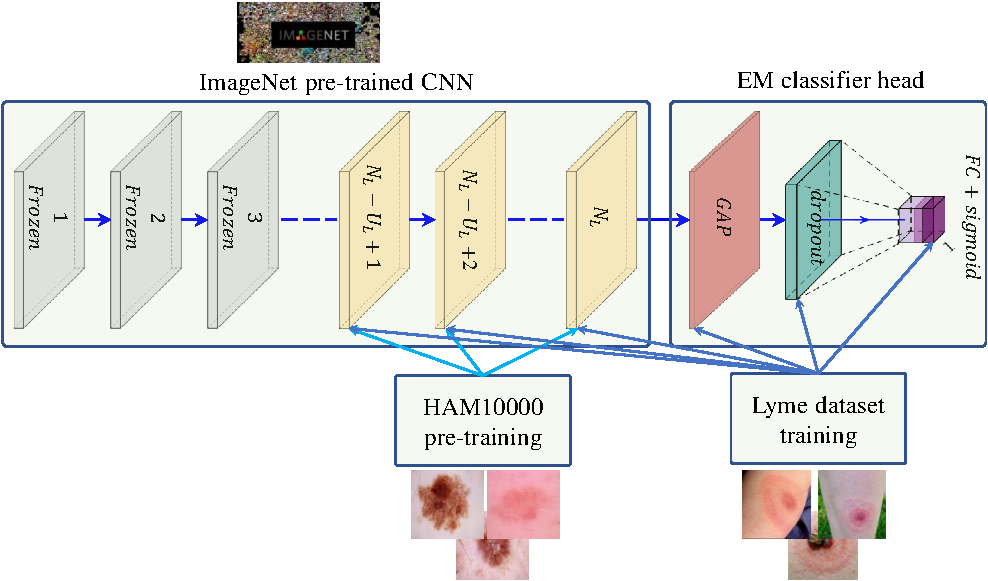
\includegraphics[width=\textwidth,keepaspectratio]{images/pretraining/pretraining-cropped.pdf}
	\caption[Pre-training strategy applied to erythema migrans  classification]{Pre-training strategy applied to erythema migrans (EM) classification. $GAP$ and $FC$ stand for global average pooling and fully connected layer respectively. $N_{L}$ is the number of ImageNet pre-trained layers and $U_{L}$ represents the number of layers used for fine-tuning. }
	\label{fig:pre-training}
\end{figure}

The intuition behind our approach is the fact that CNN mimics the ventral visual stream process of the human brain \cite{Zhuang2021}. Figure \ref{fig:ventral-stream} shows the outline of the ventral visual stream. The first visual area V1 receives optical input from the retina through the optic nerve and the lateral geniculate nucleus. V1 responds to very simple patterns (edges, lines). As the input traverses through the stream V2 and V4 respond to simple and complex shapes respectively. Further down the path inferotemporal areas respond to complex patterns of semantic entities for object understanding \cite{Qin2018}. CNNs replicate the behavior of the ventral visual stream. The initial layers of CNN learn/respond to simple patterns and the later layers respond to complex and semantic patterns. The unfrozen layers at the end of ImageNet pre-trained model giving good performance when fine-tuned on clinical skin lesion image dataset learn task-specific patterns that relate to clinical skin lesions and there should be a similarity between the skin lesion patterns of clinical and dermoscopic skin lesion images. So, fine-tuning the unfrozen part first with a dermoscopic image dataset should provide a good feature representation and weight initialization of layers for starting training with a clinical skin lesion image dataset.    
\begin{figure}[htb!]
	\centering
	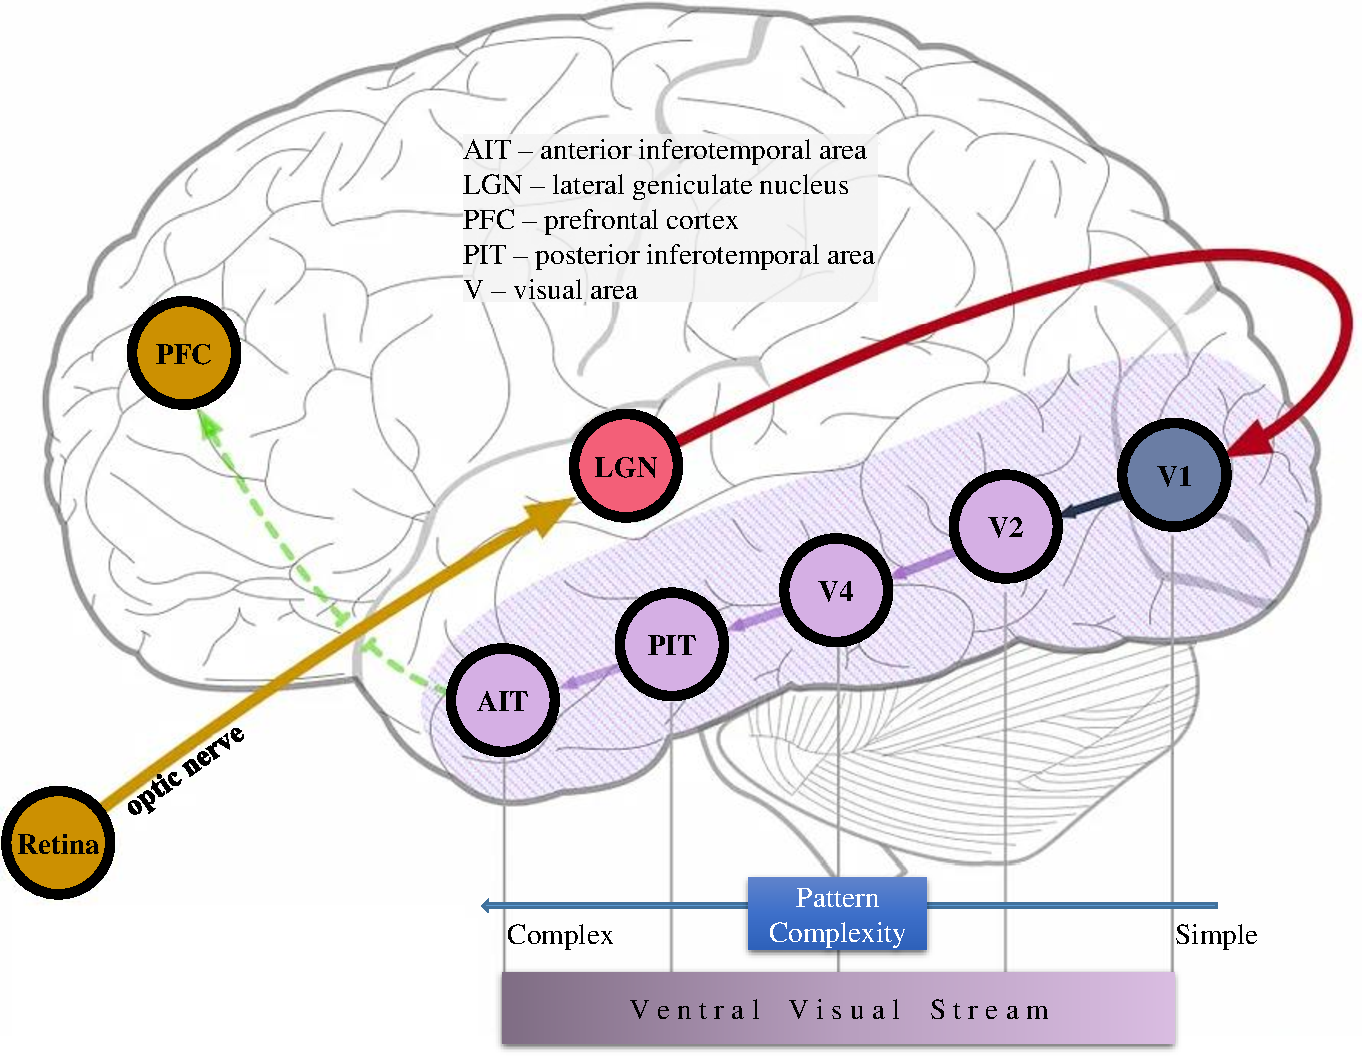
\includegraphics[width=\textwidth,keepaspectratio]{images/pretraining/ventral-stream-cropped.pdf}
	\caption[Outline of ventral visual stream]{Outline of ventral visual stream. Image modified from \cite{ventral-system}.}
	\label{fig:ventral-stream}
\end{figure}

%%%%%%%%%%%%%%%%%%%%%%%%%%%%%%%%%%%%%%%%%%%%%%%%%%%%%%%%%%%%%%%%%%%%%%%%
\subsection{Dataset Preparation}\label{sec:dataset_prep}
%%%%%%%%%%%%%%%%%%%%%%%%%%%%%%%%%%%%%%%%%%%%%%%%%%%%%%%%%%%%%%%%%%%%%%%%

As a labeled public dataset is not available for Lyme disease prediction from EM images, we created a dataset by collecting clinical skin lesion images from the internet and CF-CHU. CF-CHU collected EM images from several hospitals located in France. The use of images from the internet was inspired by related skin lesion analysis studies \cite{Burlina2018, Burlina2020, Esteva2017}. Duplicate images were removed using an image hashing-based duplicate image detector followed by the removal of inappropriate images through human inspection. After the initial curation steps, we got a total of 1672 images. Expert dermatologists and infectiologists from CF-CHU classified the curated images into two categories: EM and Confuser, making it a two-class classification problem. Out of 1672 images, 866 images were assigned to EM class and 806 images were assigned to Confuser class. The images collected from the hospitals are not shareable because of the confidentiality agreement signed with the patients. We can share images collected from the internet and the corresponding labels assigned by the doctors subject to an agreement that the images will not be made public because we do not have permission from the owners of the images \footnote{Interested researchers can send a request to dappem-project@inrae.fr for the data.}.

We further subdivided the dataset into five folds using stratified five-fold cross-validation to make sure each of the folds maintains the original class ratio. One of the folds was used as a test set and the remaining four were used as the training set with a rotation of the folds for five runs. Each time, 10\% of the training data was assigned to the validation set as shown in Figure \ref{fig:cross-validation}.
\begin{figure}[htb!]
	\centering
	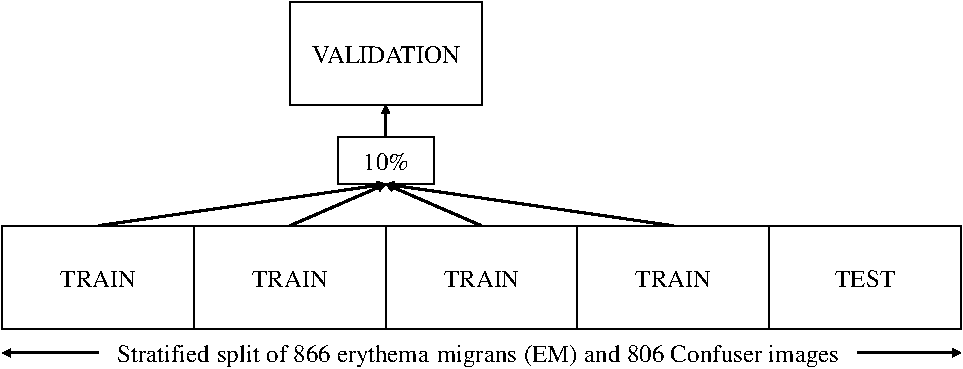
\includegraphics[width=\textwidth,keepaspectratio]{images/pretraining/cross-validation-cropped.pdf}
	\caption[Five-fold cross-validation setup]{Five-fold cross-validation setup.}
	\label{fig:cross-validation}
\end{figure}

Deep CNNs require a considerable amount of data for training and data augmentation can help with expanding the dataset. We applied data augmentation techniques only to the training images. We used flip (vertical or horizontal), rotation, brightness, contrast, and saturation augmentation by considering the best performing augmentations for skin lesions \cite{Perez2018}. Besides, we also used perspective skew transformation to cover the case of looking at a picture from different angles. Augmentor \cite{Bloice2019} an image augmentation library specially built for biomedical image augmentation was used for applying the augmentations. We used 0.5 as the probability of applying each of the augmentation operations. Rotation operation was performed with a maximum rotation angle of 5 degrees. We also used random rotation by either 90, 180, or 270 degrees. Brightness, contrast, and saturation augmentations were performed with a minimum adjustment factor of 0.7 and a maximum adjustment factor of 1.3. For all the other parameters we used default values provided by Augmentor library. The parameters were adjusted based on the visual inspection of augmented images. Figure \ref{fig:augmentation} shows some example images resulting from augmentations applied on a sample image.

\begin{figure}[htb!]
	\centering
	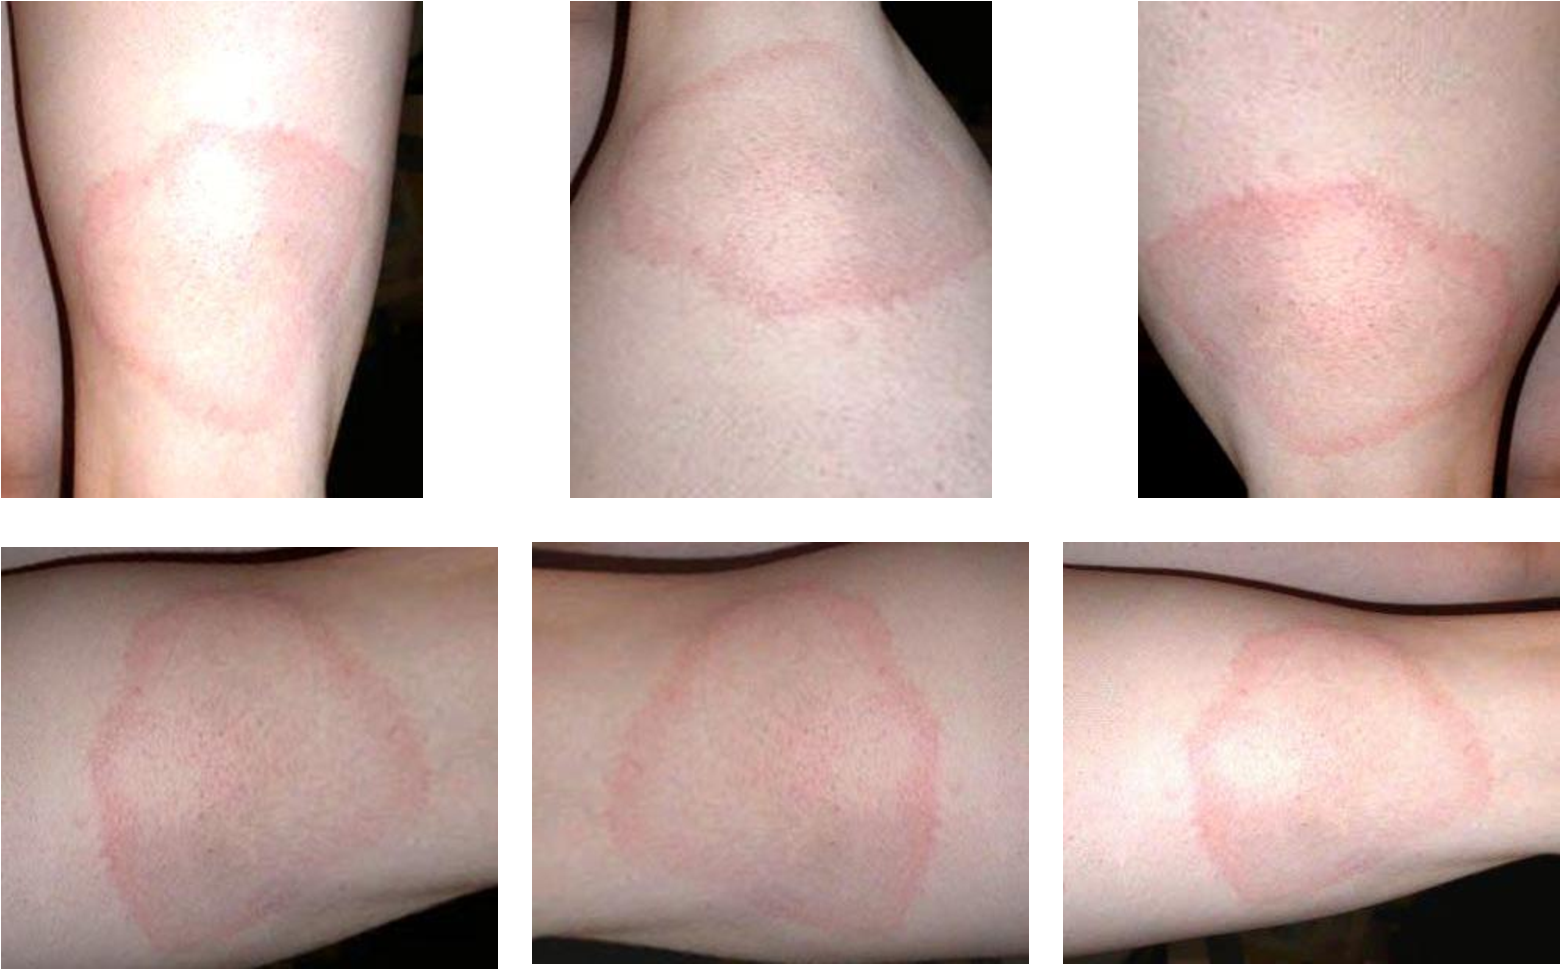
\includegraphics[width=\textwidth,keepaspectratio]{images/pretraining/Augmentation-cropped.pdf}
	\caption[Data augmentation examples]{Data augmentation examples.}
	\label{fig:augmentation}
\end{figure}

%%%%%%%%%%%%%%%%%%%%%%%%%%%%%%%%%%%%%%%%%%%%%%%%%%%%%%%%%%%%%%%%%%%%%%%%
\subsection{Brief Overview of the CNN Architectures Considered in the Study}\label{sec:CNN-archis}
%%%%%%%%%%%%%%%%%%%%%%%%%%%%%%%%%%%%%%%%%%%%%%%%%%%%%%%%%%%%%%%%%%%%%%%%
Starting with LeNet \cite{726791} in 1988 the popularity of CNNs increased with AlexNet \cite{Krizhevsky2017} winning the ImageNet large scale visual recognition challenge (ILSVRC) \cite{Russakovsky2015} of 2012. As a result of the effectiveness of CNNs in solving complex problems, several CNN architectures have been introduced over the past few years. The following subsections provide a brief overview of the CNN architectures used in this study.

%%%%%%%%%%%%%%%%%%%%%%%%%%%%%%%%%%%%%%%%%%%%%%%%%%%%%%%%%%%%%%%%%%%%%%%%
\subsubsection{VGG Architecture}
%%%%%%%%%%%%%%%%%%%%%%%%%%%%%%%%%%%%%%%%%%%%%%%%%%%%%%%%%%%%%%%%%%%%%%%%
VGG architecture \cite{Simonyan2015} is based on the idea of deeper networks with smaller filters $\left(3\times3\right)$. There are thirteen convolutional layers and three fully connected layers in VGG16 architecture as shown in Figure \ref{fig:VGG16}. Another variation of VGG architecture called VGG19 has sixteen convolutional layers and three fully connected layers. VGG architecture showed better effectiveness of deeper architectures in terms of predictive performance but requires training a huge number of parameters. 
\begin{figure}[htb!]
	\centering
	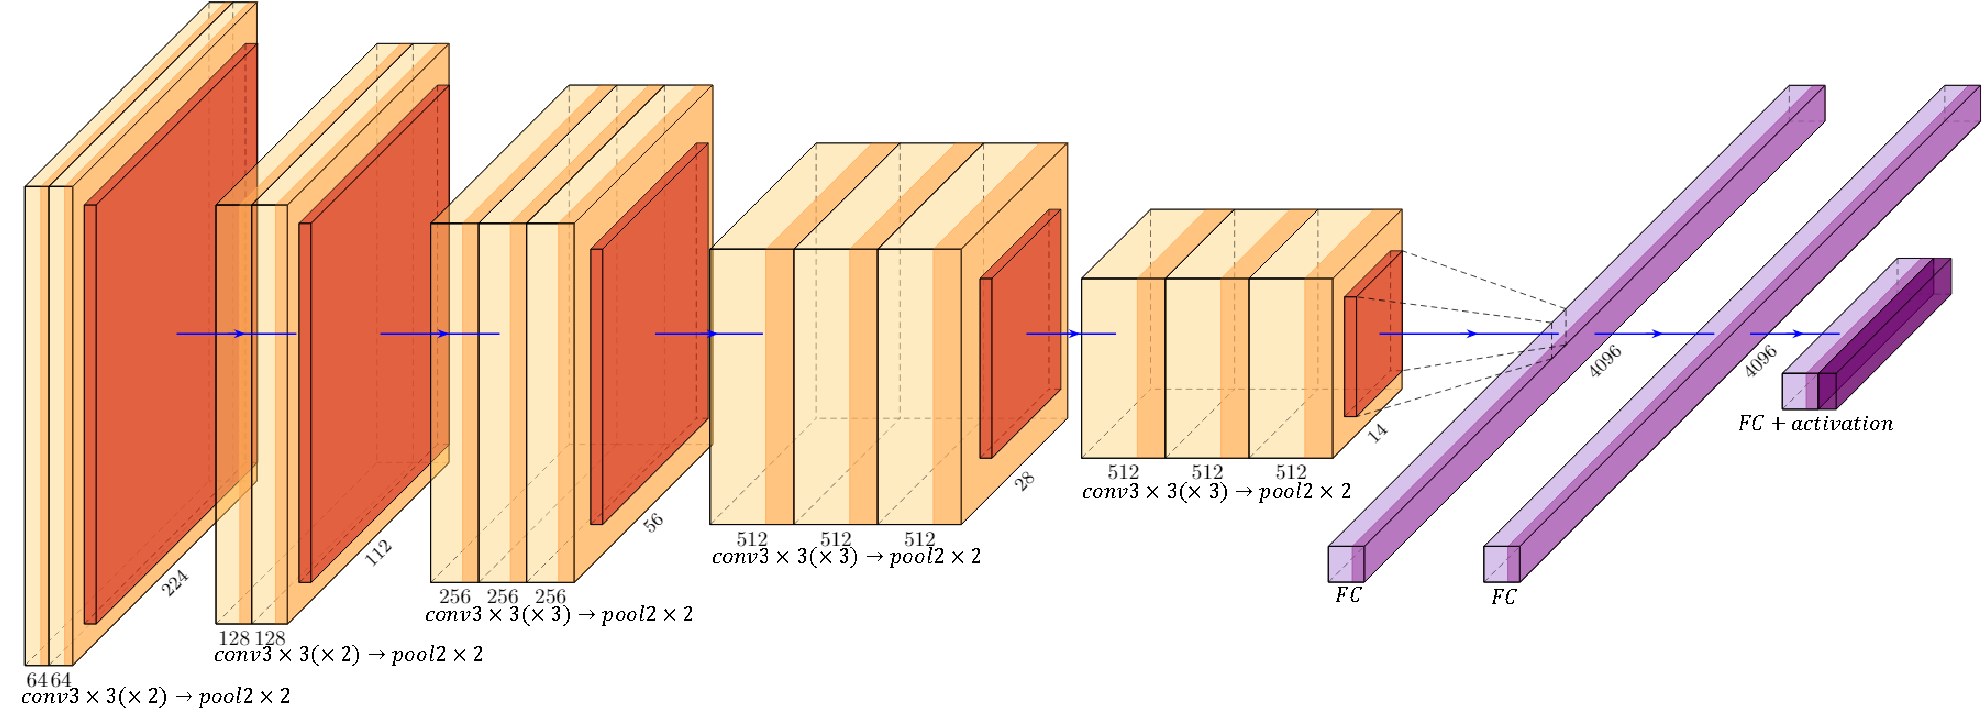
\includegraphics[width=\textwidth,keepaspectratio]{images/pretraining/VGG-cropped.pdf}
	\caption[VGG16 architecture]{VGG16 architecture. Input image is of shape $224\times224\times3$. $FC$ stands for fully connected layer.}
	\label{fig:VGG16}
\end{figure}

%%%%%%%%%%%%%%%%%%%%%%%%%%%%%%%%%%%%%%%%%%%%%%%%%%%%%%%%%%%%%%%%%%%%%%%%
\subsubsection{Inception Architecture}
%%%%%%%%%%%%%%%%%%%%%%%%%%%%%%%%%%%%%%%%%%%%%%%%%%%%%%%%%%%%%%%%%%%%%%%%
Inception architecture \cite{Szegedy2015} uses inception module as shown in Figure \ref{fig:Inception}, which is a combination of several convolution layers with small filters $\left ( 1\times1,\,3\times3,\,5\times5\right )$ applied simultaneously on the same input to facilitate the extraction of more information. The output filter banks from the convolution layers of inception module are concatenated into a single vector, which is served as the input for next stage. To reduce learnable parameters and computational complexity inception module uses $1\times1$ convolution at the beginning of convolution layers. InceptionV1 architecture is the winner of ILSVRC 2014 competition, and it’s also known as GoogleNet. Further improvement resulted in the creation of several versions of inception architectures named InceptionV2, InceptionV3, and InceptionV4 \cite{Szegedy2016, Szegedy2017}.  InceptionV2 and InceptionV3 improved the architecture with smart factorized convolution, batch normalized auxiliary classifier, and label smoothing whereas, InceptionV4 focused on the uniformity of the architecture with more inception modules than InceptionV3.
\begin{figure}[htb!]
	\centering
	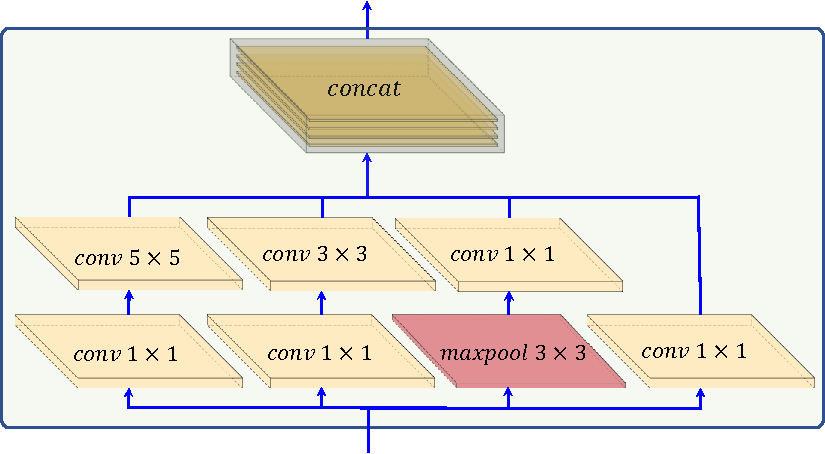
\includegraphics[width=\textwidth,keepaspectratio]{images/pretraining/Inception-cropped.pdf}
	\caption[Inception module of Inception architecture]{Inception module of Inception architecture. \enquote{concat} represents the concatenation of feature maps.}
	\label{fig:Inception}
\end{figure}

%%%%%%%%%%%%%%%%%%%%%%%%%%%%%%%%%%%%%%%%%%%%%%%%%%%%%%%%%%%%%%%%%%%%%%%%
\subsubsection{ResNet Architecture}
%%%%%%%%%%%%%%%%%%%%%%%%%%%%%%%%%%%%%%%%%%%%%%%%%%%%%%%%%%%%%%%%%%%%%%%%
ResNet architecture \cite{He2016} tried to solve the vanishing gradient and accuracy degradation problems of deep models by introducing residual block with identity shortcut connection that directly connects the input to the output of the block allowing the gradient to flow through the shortcut path as shown in Figure \ref{fig:resnet}. It’s the winner of ILSVRC 2015 competition. Depending on the number of weight layers there are many variants of ResNet architecture such as ResNet18, ResNet34, ResNet50, ResNet101, ResNet152, ResNet164, ResNet1202, etc., where the number represents the count of weight layers. Deeper ResNet architectures use bottleneck blocks where 3x3 convolution is sandwiched between $1\times1$ convolutions, responsible for transitory reduction and expansion of channels.  The $wide\rightarrow narrow \rightarrow wide$ architecture of bottlenecks reduces multiplications and the number of parameters and helps the network grow deeper with fewer parameters. He et al. \cite{He2016a} proposed ResNetV2 with pre-activation of the weight layers as opposed to the post-activation of original ResNet architecture.  InceptionResNet is a hybrid of Inception and ResNet architecture having two variations named InceptionResNetV1 and InceptionResNetV2, which differ mainly in terms of the number of used filters \cite{Szegedy2017}. Liu et al. \cite{ConvNeXtRef} modernized ResNet architecture to match the performance of vision transformers resulting in a new family of architectures called ConvNeXt. ConvNeXt utilizes inverted bottleneck ( $narrow\rightarrow wide \rightarrow narrow$), large kernel, depthwise convolution (shown in Figure \ref{fig:depthwise}), layer normalization \cite{LayerNormRef} instead of batch normalization \cite{BatchNormref}, and GELU activation ReLU as compared to base ResNet models.
\begin{figure}[htb!]
	\centering
	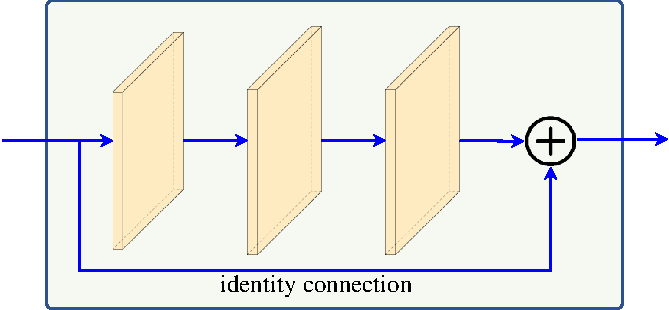
\includegraphics[width=0.5\textwidth,keepaspectratio]{images/pretraining/ResNet-cropped.pdf}
	\caption[Residual block of ResNet architecture]{Residual block of ResNet architecture.}
	\label{fig:resnet}
\end{figure}

%%%%%%%%%%%%%%%%%%%%%%%%%%%%%%%%%%%%%%%%%%%%%%%%%%%%%%%%%%%%%%%%%%%%%%%%
\subsubsection{DenseNet Architecture}
%%%%%%%%%%%%%%%%%%%%%%%%%%%%%%%%%%%%%%%%%%%%%%%%%%%%%%%%%%%%%%%%%%%%%%%%
Dense Convolutional Network (DenseNet) \cite{DenseNetRef} extended ResNet by introducing dense blocks where each layer within a dense block receives inputs from all the previous layers as shown in Figure \ref{fig:densenet} DenseNet concatenates the incoming feature maps of a layer with output feature maps instead of summing them up as done in ResNet. Dense blocks within DenseNet are connected with transition layers consisting of convolution and pooling to perform the required downsampling operation. Depending on the number of weight layers there are several versions of DenseNet like DenseNet121, DenseNet169, DenseNet201, DenseNet264, etc. Besides solving the vanishing gradient problem DenseNet also eases feature propagation and reuse, and a reduction in the number of learnable parameters compared to ResNet.
\begin{figure}[htb!]
	\centering
	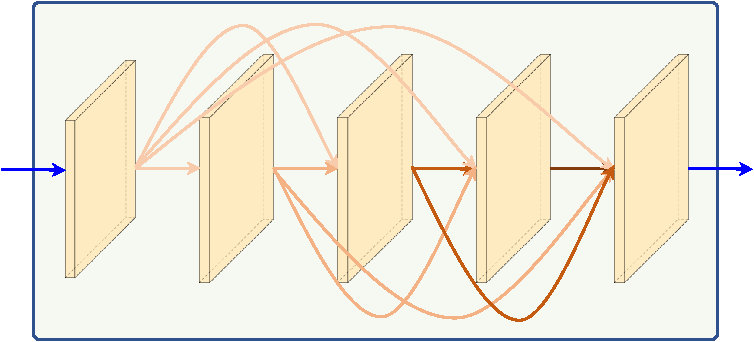
\includegraphics[width=0.6\textwidth,keepaspectratio]{images/pretraining/dense-cropped.pdf}
	\caption[Building block of DenseNet architecture]{Building block of DenseNet architecture.}
	\label{fig:densenet}
\end{figure}

%%%%%%%%%%%%%%%%%%%%%%%%%%%%%%%%%%%%%%%%%%%%%%%%%%%%%%%%%%%%%%%%%%%%%%%%
\subsubsection{MobileNet Architecture}
%%%%%%%%%%%%%%%%%%%%%%%%%%%%%%%%%%%%%%%%%%%%%%%%%%%%%%%%%%%%%%%%%%%%%%%%
MobileNetV1 \cite{Howard2017} used depthwise separable convolution extensively to reduce the computational cost. Standard convolution performs spatial and channel-wise computations in one step but depthwise separable convolution first applies separate convolutional filter for each input channel and then uses pointwise convolution on concatenated channels to produce required number of output channels as shown in Figure \ref{fig:depthwise}. MobileNetV1 was designed to run very efficiently on mobile and embedded devices. MobileNetV2 \cite{Sandler2018} improved upon the concepts of MobileNetV1 by incorporating thin linear bottlenecks with shortcut connections between the bottlenecks as shown in Figure \ref{fig:mobilenetv2}. This is called inverted residual block as it uses $narrow\rightarrow wide \rightarrow narrow$ as opposed to the $wide\rightarrow narrow \rightarrow wide$ architecture of traditional residual block. MobileNetV3 \cite{Howard2019} incorporated squeeze-and-excitation layers \cite{Hu2020} in the building block of MobileNetV2 which provides channel-wise attention and used MnasNet \cite{Tan2019} to search for a coarse architecture that was further optimized with NetAdapt \cite{Yang2018} algorithm.
\begin{figure}[htb!]
	\centering
	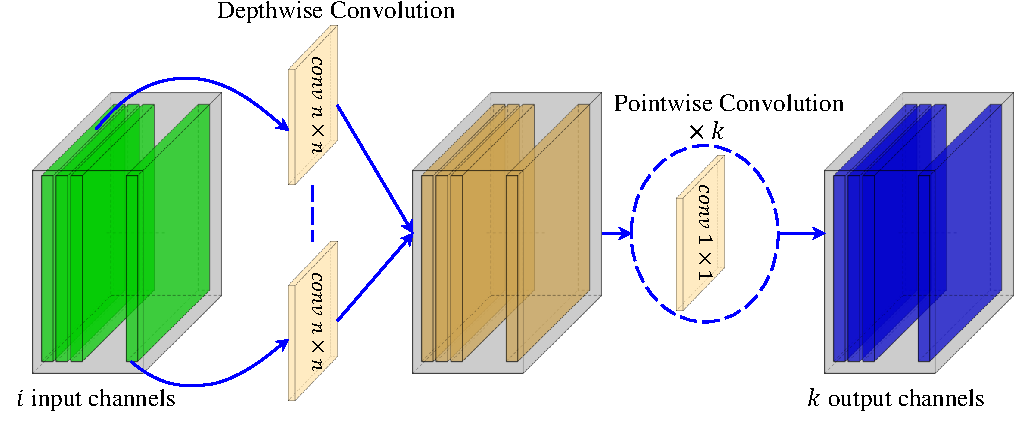
\includegraphics[width=\textwidth,keepaspectratio]{images/pretraining/depthwise-cropped.pdf}
	\caption[Depthwise separable convolution]{Depthwise separable convolution.}
	\label{fig:depthwise}
\end{figure}
\begin{figure}[htb!]
	\centering
	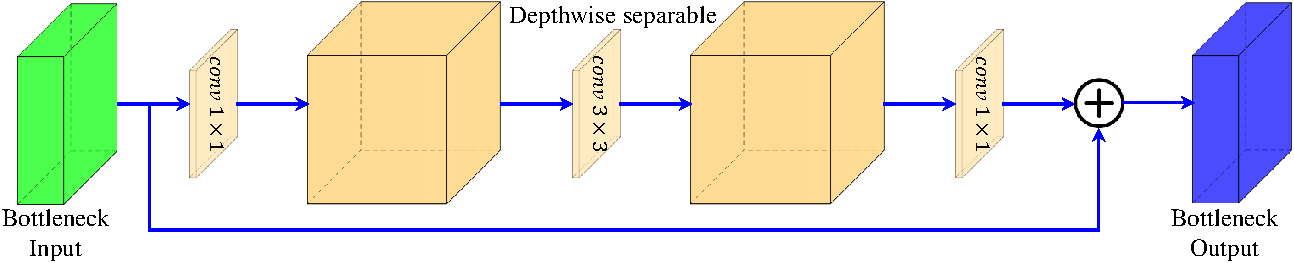
\includegraphics[width=\textwidth,keepaspectratio]{images/pretraining/mnetv2-cropped.pdf}
	\caption[Building block of MobileNetV2 architecture]{Building block of MobileNetV2 architecture.}
	\label{fig:mobilenetv2}
\end{figure}

%%%%%%%%%%%%%%%%%%%%%%%%%%%%%%%%%%%%%%%%%%%%%%%%%%%%%%%%%%%%%%%%%%%%%%%%
\subsubsection{Xception Architecture}
%%%%%%%%%%%%%%%%%%%%%%%%%%%%%%%%%%%%%%%%%%%%%%%%%%%%%%%%%%%%%%%%%%%%%%%%
Extreme version of Inception the Xception architecture \cite{XceptionRef} replaced the Inception module with a modified version of depthwise separable convolution where the order of depthwise convolution and pointwise convolutions are reversed as shown in Figure \ref{fig:xception}. Xception also uses shortcut connections like ResNet architecture. On ImageNet dataset Xception performs slightly better than the InceptionV3 architecture.
\begin{figure}[htb!]
	\centering
	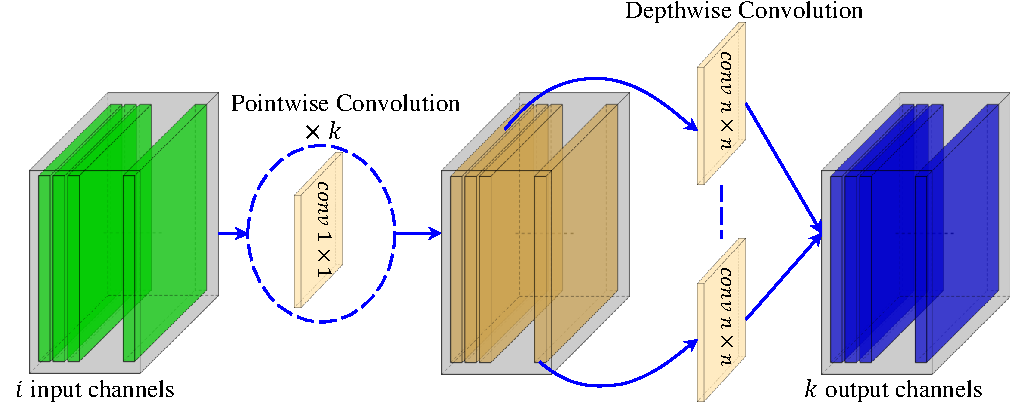
\includegraphics[width=\textwidth,keepaspectratio]{images/pretraining/pointwise-cropped.pdf}
	\caption[Building block of Xception architecture]{Building block of Xception architecture.}
	\label{fig:xception}
\end{figure}

%%%%%%%%%%%%%%%%%%%%%%%%%%%%%%%%%%%%%%%%%%%%%%%%%%%%%%%%%%%%%%%%%%%%%%%%
\subsubsection{NASNet Architecture}
%%%%%%%%%%%%%%%%%%%%%%%%%%%%%%%%%%%%%%%%%%%%%%%%%%%%%%%%%%%%%%%%%%%%%%%%
Neural Architecture Search Netowork \cite{NASnetref} from Google Brain utilizes reinforcement learning with a Recurrent Neural Network based controller to search for efficient building blocks for a smaller dataset which is then transferred to a larger dataset by stacking multiple copies of the found building block.  NASNet blocks are comprised of normal and reduction cells as shown in Figure \ref{fig:NASnet}. Normal cells produce feature maps of the same size as input whereas reduction cells reduce the size by a factor of two. NASNet optimized for mobile applications is called NASNetMobile whereas the larger version is called NASNetLarge.
\begin{figure}[htb!]
	\centering
	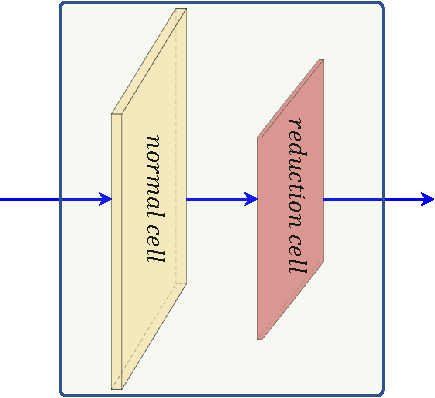
\includegraphics[width=0.4\textwidth,keepaspectratio]{images/pretraining/NASnet-cropped.pdf}
	\caption[Building block of NASNet architecture]{Building block of NASNet architecture.}
	\label{fig:NASnet}
\end{figure}

%%%%%%%%%%%%%%%%%%%%%%%%%%%%%%%%%%%%%%%%%%%%%%%%%%%%%%%%%%%%%%%%%%%%%%%%
\subsubsection{EfficientNet Architecture}
%%%%%%%%%%%%%%%%%%%%%%%%%%%%%%%%%%%%%%%%%%%%%%%%%%%%%%%%%%%%%%%%%%%%%%%%
EfficientNet \cite{efficientNetRef} which is among the most efficient models proposed a scaling method to uniformly scale all dimensions of a network using a compound coefficient. The baseline network of EfficientNet was built with NAS incorporating squeeze-and-excitation in the building block of MobileNetV2. EffcientNet’s building block also called MBConv is shown in Figure \ref{fig:MBConv}.
\begin{figure}[htb!]
	\centering
	\begin{subfigure}[b]{\textwidth}
		\centering
		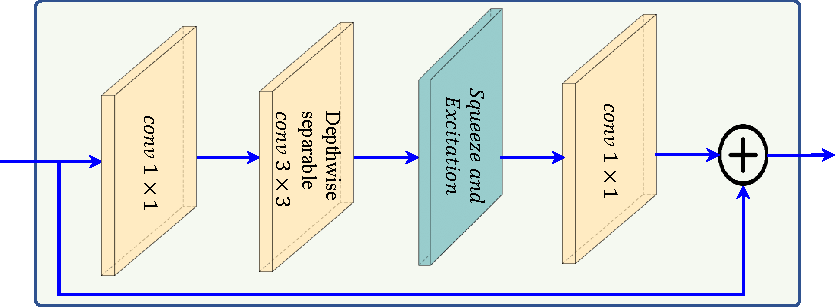
\includegraphics[width=\textwidth,keepaspectratio]{images/pretraining/MBConv-cropped.pdf}
		\caption{MBConv block.}
		\label{fig:MBConv}
	\end{subfigure}
	\hfill
	\begin{subfigure}[b]{0.75\textwidth}
		\centering
		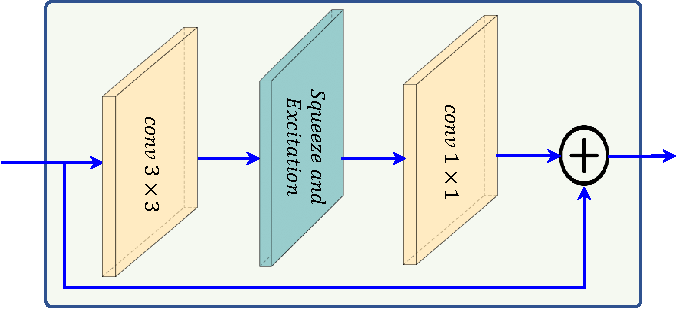
\includegraphics[width=\textwidth,keepaspectratio]{images/pretraining/FusedMBConv-cropped.pdf}
		\caption{Fused-MBConv block.}
		\label{fig:Fused-MBConv}
	\end{subfigure}
	
	\caption{EfficientNet building blocks.}
	\label{fig:mobilenet-blocks}
\end{figure}
The scaling method is defined as:
\begin{gather*}
	depth=\zeta_{1}^{\Theta}\\
	width=\zeta_{2}^{\Theta}\\
	resolution=\zeta_{3}^{\Theta}\\
	s.t.\; \zeta_{1}.\zeta_{2}^{2}.\zeta_{3}^{2}\approx2;\,\zeta_{1}\geq1,\zeta_{2}\geq1,\zeta_{1}\geq1
\end{gather*}
where, the coefficient $\Theta$ controls available resources and $\zeta_{1},\zeta_{2}$, and $\zeta_{3}$ are constants obtained by grid search. EfficientNetB0-B7 are a family of architectures scaled up from the baseline network that reflects a good balance of accuracy and efficiency. EfficientV2 was designed to optimize parameter efficiency and training speed. It used an additional Fused-MBConv block. Fused-MBConv uses $3\times3$ convolution instead of the $3\times3$ depthwise and $1\times1$ convolutions of MBConv as shown in Figure \ref{fig:Fused-MBConv}. Although Fused-MBConv adds a small overhead it improves training speed compared to MBConv. EfficientV2 used training-aware NAS to find the best combination of MBConv and Fused-MBConv blocks. 

%%%%%%%%%%%%%%%%%%%%%%%%%%%%%%%%%%%%%%%%%%%%%%%%%%%%%%%%%%%%%%%%%%%%%%%%
\subsection{Predictive Performance Measures}
%%%%%%%%%%%%%%%%%%%%%%%%%%%%%%%%%%%%%%%%%%%%%%%%%%%%%%%%%%%%%%%%%%%%%%%%
To compare the predictive performance of the trained CNN models we used accuracy, recall/sensitivity/hit rate/true positive rate (TPR), specificity/selectivity/true negative rate (TNR), precision/ positive predictive value (PPV), negative predictive value (NPV), Cohen’s kappa coefficient ($\kappa$), Matthews correlation coefficient (MCC), positive likelihood ratio (LR$+$), negative likelihood ratio (LR$-$), F1-score, confusion matrix and area under the receiver operating characteristic (ROC) curve (AUC) metrics. Confusion matrix is a way of presenting the count of true negatives (TN), false positives (FP), false negatives (FN), and true positives (TP) in a matrix format where the y-axis presents true labels and x-axis presents predicted labels. Accuracy measures the proportion of correctly classified predictions among all the predictions, and it is calculated as:
\begin{equation}
	Accuracy =\frac{TP+TN}{TP+TN+FP+FN}
\end{equation}
Recall/sensitivity/hit rate/TPR measures the proportion of actual positives correctly identified, and it is expressed as:
\begin{equation}
	Recall,\, Sensitivity,\, hit rate,\, T P R=\frac{T P}{T P+F N}
\end{equation}
Specificity/selectivity/ TNR measures the proportion of actual negatives correctly identified, and it is expressed as:
\begin{equation}
	Specificity,\, Selectivity,\, TNR =\frac{T N}{T N+F P}
\end{equation}
Precision/ PPV measures the proportion of correct positive predictions, and it is calculated as:
\begin{equation}
	Precision,\, P P V=\frac{T P}{T P+F P}
\end{equation}
NPV measures the proportion of negative predictions that are correct, and it is calculated as:
\begin{equation}
	N P V=\frac{T N}{T N+F N}
\end{equation}
MCC provides a summary of the confusion matrix, and it is calculated as:
\begin{equation}
	M C C=\frac{T P * T N-F P * F N}{\sqrt{(T P+F P)(T P+F N)(T N+F P)(T N+F N)}}
\end{equation}
MCC value is in the range $\left[ -1,+1\right]$, where 0 is like random prediction, $+1$ means a perfect prediction, and $-1$ represents inverse prediction. Cohen’s kappa coefficient ($\kappa$) metric is used to assess inter-rater agreement which tells us how the model is performing compared to a random classifier, and it is calculated with the formula:
\begin{equation}
	\kappa=\frac{p_o-p_e}{1-p_e}
\end{equation}
where $p_o$ is the relative observed agreement among the raters and $p_e$ is the hypothetical probability of expected agreement which is defined for $c$ categories as:
\begin{equation}
	p_e=\frac{1}{N^2} \sum_c n_{c 1} n_{c 2}
\end{equation}
where, $N$ is the total number of observations, and $n_{cr}$ is the number of predictions of category $c$ by rater $r$. The value of $\kappa$ is in the range $\left[ -1,+1\right]$, where a value of 1 indicates perfect agreement, 0 means agreement only by chance, and a negative value indicates the agreement is worse than the agreement by chance. Likelihood ratio (LR) is used for assessing the potential utility of performing a diagnostic test and it is calculated for both positive test and negative test results called LR$+$ and LR$-$, respectively. LR$+$ is the ratio of the probability of a person having a disease testing positive to the probability of a person without the disease testing positive. LR$-$ is the ratio of the probability of a person having the disease testing negative to the probability of without the disease testing negative. LR$+$ and LR$-$ are calculated based on sensitivity and specificity values using the following formulas:
\begin{equation}
	LR+ =\frac{sensitivity}{1-specificity}
\end{equation}
\begin{equation}
	LR- =\frac{1-sensitivity}{specificity}
\end{equation}
A value of LR greater than 1 shows increased evidence. F1-Score combines precision and recall, and it is defined as the harmonic mean of precision and recall as follows:
\begin{equation}
	F1-Score=2 * \frac{ Precision  *  Recall }{Precision+ Recall}
\end{equation}
ROC curve is a plot of TPR against false positive rate (FPR) at various threshold settings where FPR is defined as: 
\begin{equation}
	FPR =\frac{FP}{FP+TN}
\end{equation}
Area under the ROC curve (AUC) is the measure of the classifier’s ability to separate between classes and the higher the AUC, the better the ability of the classifier for separating the positive class from the negative class. As our dataset is balanced so, accuracy can be considered a good measure of predictive performance \cite{Chicco2020} and we did most of the analysis in terms of accuracy but also kept the other metrics to provide insights for experts from different domains as done in relevant studies \cite{Burlina2018,Burlina2020}. 

We have used critical difference (CD) diagram \cite{Demsar2006} to rank the CNN models in terms of accuracy and to show the statistically significant difference in predictive performance. A thick horizontal line connects a group of models in the CD diagram that are not significantly different in terms of predictive performance. We used non-parametric Friedman test \cite{Friedman1940} to reject the null hypothesis of statistical similarity among all the models followed by Nemenyi post-hoc all-pair comparison test \cite{Nemenyi1963} for showing the difference among the models at a significance level, $\alpha=0.1$. Although deep CNN architectures often do not show any statistically significant differences when tested on large and small image datasets \cite{Burlina2020, Zoph2018, Khan_2020}, CD diagram is a good way to visualize the multi-fold rank comparisons of the models.

%%%%%%%%%%%%%%%%%%%%%%%%%%%%%%%%%%%%%%%%%%%%%%%%%%%%%%%%%%%%%%%%%%%%%%%%
\subsection{Model Complexity Measures}
%%%%%%%%%%%%%%%%%%%%%%%%%%%%%%%%%%%%%%%%%%%%%%%%%%%%%%%%%%%%%%%%%%%%%%%%
To compare the trained CNNs in terms of complexity we used the total number of model parameters, the total number of floating-point operations (FLOPs), average training time per epoch, GPU memory usage, and average inference time per image. FLOPs reveal how computationally costly a model is and we counted FLOPs for each of the models using TensorFlow profiler [47] considering a batch size of one.  For reporting the average training time per epoch, we calculated the average of the training time of three epochs during transfer learning fine-tuning. We calculated the GPU memory usage of a CNN model by inspecting the memory allocated in the GPU after loading a trained instance of the model. To measure the average inference time per image of a model we took the average of three hundred inferences on the same input image.

%%%%%%%%%%%%%%%%%%%%%%%%%%%%%%%%%%%%%%%%%%%%%%%%%%%%%%%%%%%%%%%%%%%%%%%%
\section{Experimental Studies}\label{sec:exp_result_pretrain}
%%%%%%%%%%%%%%%%%%%%%%%%%%%%%%%%%%%%%%%%%%%%%%%%%%%%%%%%%%%%%%%%%%%%%%%%
The following subsections describe experimental settings including model selection and parameter settings, software and hardware used for the study, the experimental results, and recommendations for model selection.

%%%%%%%%%%%%%%%%%%%%%%%%%%%%%%%%%%%%%%%%%%%%%%%%%%%%%%%%%%%%%%%%%%%%%%%%
\subsection{Experimental Settings}\label{sec:exp_settings}
%%%%%%%%%%%%%%%%%%%%%%%%%%%%%%%%%%%%%%%%%%%%%%%%%%%%%%%%%%%%%%%%%%%%%%%%
We did an extensive analysis using the ResNet50 architecture to see the effectiveness of our proposed pre-training strategy (described in Section \ref{sec:pretraining-strag}) on the novel Lyme disease dataset. For this purpose, we tested different configurations:
\begin{enumerate}[i.]
	
	\item Training ResNet50 model on our Lyme dataset from scratch without using transfer learning (called ResNet50-NTL, where, NTL stands for no transfer learning).
	
	\item Pre-training ResNet50 model with only HAM10000 data followed by fine-tuning all the layers with our Lyme dataset (called ResNet50-HAM-FFT, where HAM means HAM10000 and FFT stands for full fine-tuning).
	
	\item Training only the EM classifier head of an ImageNet pre-trained ResNet50 model with our Lyme dataset (called ResNet50-IMG-WFT, where IMG means ImageNet and WFT stands for without fine-tuning).
	
	\item Fine-tuning all the layers of ImageNet pre-trained ResNet50 model with our Lyme dataset (called ResNet50-IMG-FFT).
	
	\item Fine-tuning $U_L$ number of layers of an ImageNet pre-trained ResNet50 model with our Lyme dataset (called ResNet50-IMG-FT$U_L$, where FT${U_L}$ means fine-tuning $U_L$ number of layers).
	
	\item Pre-training the whole ImgaeNet pre-trained ResNet50 model by HAM10000 data before fine-tuning $U_L$ layers with our Lyme dataset (called ResNet50-IMG-HAMFP-FT$U_L$, where, HAMFP means full pre-training with HAM10000 dataset).
	
	\item Pre-training only the unfrozen $U_L$ layers of a ImgaeNet pre-trained ResNet50 model with HAM10000 data before fine-tuning $U_L$ layers with our Lyme dataset (called  ResNet50-IMG-HAMPP-FT$U_L$, where, HAMPP means partial pre-training with HAM10000 dataset). This setting corresponds to \textbf{our proposed pre-training strategy} (described in Section \ref{sec:pretraining-strag}).
	
	\item To see the effect of data augmentation, we trained a ResNet50 model without data augmentation and transfer learning (called ResNet50-NoAug, where NoAug means no data augmentation). All the other configurations were trained with data augmentation as described in Section \ref{sec:dataset_prep}. 
\end{enumerate}
According to the experimental results (discussed in Section \ref{sec:pretrain-results}), our proposed pre-training configuration ResNet50-IMG-HAMPP-FT$U_L$ performed best, and we used this configuration for training twenty-five well-known CNNs to find out the effective architecture for diagnosing Lyme disease from EM images. For this benchmarking we trained VGG16\footnote{ImageNet pre-trained model taken from \url{https://www.tensorflow.org/api_docs/python/tf/keras/applications} (visited on 02/20/2023).\label{note:model_download}}, VGG19\footref{note:model_download}, ResNet50\footref{note:model_download}, ResNet101\footref{note:model_download}, ResNet50V2\footref{note:model_download}, ResNet101V2\footref{note:model_download}, InceptionV3\footref{note:model_download}, InceptionV4\footref{note:model_download}, InceptionResNetV2\footref{note:model_download}, Xception\footref{note:model_download}, DenseNet121\footref{note:model_download}, DenseNet169\footref{note:model_download}, DenseNet201\footref{note:model_download}, MobileNetV2\footref{note:model_download}, MobileNetV3Large\footref{note:model_download}, MobileNetV3Small\footref{note:model_download}, NASNetMobile\footref{note:model_download}, EfficientNetB0\footref{note:model_download}, EfficientNetB1\footref{note:model_download}, EfficientNetB2\footref{note:model_download}, EfficientNetB3\footref{note:model_download}, EfficientNetB4\footref{note:model_download}, EfficientNetB5\footref{note:model_download}, EfficientNetV2S\footref{note:model_download} and ConvNextTiny\footref{note:model_download} architectures. These models were selected to explore a diverse set of CNN models covering various prospects, like different architectures, depths, and complexities. For simplicity, the best performing trained models of each of the architectures are presented in ModelName-U$U_L$ format, where $U_L$ represents the number of unfrozen layers. For example, EfficientNetB0-187 means EfficientNetB0-IMG-HAMPP-FT187 and ResNet50-141 means ResNet50-IMG-HAMPP-FT141. To the best of our knowledge, ResNet50 is the only publicly available trained CNN that was used for Lyme disease identification by Burlina et al. \cite{Burlina2018}. We are calling this model ResNet50-Burlina which is a collection of five models (trained on five-fold cross-validation data)\footnote{\url{https://github.com/neil454/lyme-1600-model} (visited on 02/20/2023).}.

For training all the models, we used a dropout rate of 0.2 for the dropout layer in EM classifier head section. Adam optimizer (described in Appendix Section \ref{app:optimizer}) with author-recommended default values for parameters was used with a learning rate of 0.0001 for training the classifier head and 0.00001 for fine-tuning. We also used early stopping to terminate the training if there was no improvement in validation accuracy for ten epochs. A batch size of 32 was used. For reporting the number of layers to unfreeze during transfer learning, we stated the total number of layers to unfreeze including layers containing both trainable and non-trainable parameters.

We used NVIDIA QUADRO RTX 8000 GPU and a Desktop Computer with Intel Xeon W-2175 processor, 64 GB DDR4 RAM, and Ubuntu 18.04 operating system to perform all the experiments. Python v3.6.9, and TensorFlow v2.4.1 platform \cite{Abadi2016} were used for all the implementations and experiments of this study.

%%%%%%%%%%%%%%%%%%%%%%%%%%%%%%%%%%%%%%%%%%%%%%%%%%%%%%%%%%%%%%%%%%%%%%%%
\subsection{Results and Discussion}\label{sec:pretrain-results}
%%%%%%%%%%%%%%%%%%%%%%%%%%%%%%%%%%%%%%%%%%%%%%%%%%%%%%%%%%%%%%%%%%%%%%%%
Table \ref{tab:ResNet50-results} presents the predictive performance measures of our eight different configurations (explained in Section \ref{sec:exp_settings}). ResNet50-NoAug model resulting from training a ResNet50 architecture from scratch without using data augmentation and transfer learning gave an accuracy of 61.42\%. ResNet50-NTL model obtained by training ResNet50 architecture with data augmentation and without transfer learning improved the accuracy to 76.35\%. So, data augmentation provided large gain in predictive performance (ResNet50-NTL compared to ResNet50-NoAug). ResNet50-HAM-FFT model resulting from pretraining ResNet50 architecture with only HAM10000 data followed by fine-tuning of all the layers with our Lyme dataset showed a degraded accuracy of 72.27\%. ResNet50-IMG-WFT, generated by training only the EM classifier head of an ImageNet pre-trained ResNet50 architecture improved the accuracy to 78.94\%. ResNet50-IMG-FFT, resulting from fine-tuning all the layers of ImageNet pre-trained ResNet50 architecture, further improved the classification accuracy to 82.22\%. Whereas ResNet50-IMG-FT141, model resulting from fine-tuning 141 layers of pre-trained ResNet50 architecture gave an accuracy of 83.24\% which is better compared to unfreezing the full architecture. ResNet50-IMG-HAMFP-FT141, model resulting from pretraining the whole ImgaeNet pre-trained ResNet50 model by HAM10000 data before fine-tuning 141 layers with our Lyme dataset reduced the accuracy to 82.35\%. Our proposed pre-training strategy(described in Section \ref{sec:pretraining-strag}) i.e. pre-training only the unfrozen 141 layers with HAM10000 data gave us the model ResNet50-IMG-HAMPP-FT141 with the best accuracy of 84.42\%. Figure \ref{fig:CD_ResNet} shows the CD diagram in terms of accuracy for these ResNet50 based models. The Friedman test null hypothesis was rejected with a $p$ value of 0.00003. From the CD diagram, we can see that ResNet50-IMG-HAMPP-FT141 achieved the best average ranking among the compared models. Although there is no statistically significant difference among ResNet50-IMG-FFT, ResNet50-IMG-FT141, ResNet50-IMG-HAMFP-FT141, and ResNet50-IMG-HAMPP-FT141 in terms of accuracy the ResNet50-IMG-HAMPP-FT141 model performed better in terms of most of the metrics (7 out of 11) as highlighted in Table \ref{tab:ResNet50-results}. To summarize, our proposed  strategy of pre-training only the unfrozen part of an ImageNet pre-trained CNN with HAM10000 data provided the best accuracy according to our experiments. So, for benchmarking all the other CNN architectures, we only reported the performance resulting from this configuration.

\begin{table}[tbh!]
	\centering
	\caption[Five-fold cross-validation performance metrics of ResNet50 based configurations]{Five-fold cross-validation performance metrics of ResNet50 based configurations. Within each cell, the value after $\pm$ symbol represents the standard deviation across five folds. Bold indicates the best result for each of the metrics.}
	\label{tab:ResNet50-results}
	\resizebox{\textwidth}{!}{%
		\begin{tabular}{llllllllllll}
			\toprule
			& \multicolumn{11}{c}{\textbf{Metric}}    \\ \cmidrule(l){2-12} 
			\multicolumn{1}{c}{\textbf{Model}} & \rotatebox{45}{Accuracy} & \rotatebox{45}{Sensitivity} & \rotatebox{45}{Specificity} & \rotatebox{45}{Precision} & \rotatebox{45}{NPV} & \rotatebox{45}{MCC} & \rotatebox{45}{Kappa} & \rotatebox{45}{LR$+$} & \rotatebox{45}{LR$-$} & \rotatebox{45}{F1-Score} & \rotatebox{45}{AUC}  \\ \midrule
			\begin{tabular}[c]{@{}l@{}}ResNet50-\\NoAug\end{tabular} & \begin{tabular}[c]{@{}l@{}}61.42\\ $\pm$1.29\end{tabular}  & \begin{tabular}[c]{@{}l@{}}71.73\\ $\pm$8.65\end{tabular} & \begin{tabular}[c]{@{}l@{}}50.37\\ $\pm$8.79\end{tabular} & \begin{tabular}[c]{@{}l@{}}61.0\\ $\pm$1.5\end{tabular} & \begin{tabular}[c]{@{}l@{}}63.03\\ $\pm$3.17\end{tabular} & \begin{tabular}[c]{@{}l@{}}0.2302\\ $\pm$0.0234\end{tabular} & \begin{tabular}[c]{@{}l@{}}0.2224\\ $\pm$0.0256\end{tabular} & \begin{tabular}[c]{@{}l@{}}1.4592\\ $\pm$0.0863\end{tabular} & \begin{tabular}[c]{@{}l@{}}0.5497\\ $\pm$0.0764\end{tabular} & \begin{tabular}[c]{@{}l@{}}0.656\\ $\pm$0.0325\end{tabular} & \begin{tabular}[c]{@{}l@{}}0.6505\\ $\pm$0.0216\end{tabular} \\ 
			\cmidrule(lr){1-12}
			
			ResNet50-NTL & \begin{tabular}[c]{@{}l@{}}76.35\\ $\pm$2.43\end{tabular}  & \begin{tabular}[c]{@{}l@{}}78.49\\ $\pm$8.47\end{tabular}  & \begin{tabular}[c]{@{}l@{}}74.04\\ $\pm$4.6\end{tabular}  & \begin{tabular}[c]{@{}l@{}}76.64\\ $\pm$1.64\end{tabular}  & \begin{tabular}[c]{@{}l@{}}76.92\\ $\pm$5.22\end{tabular}  & \begin{tabular}[c]{@{}l@{}}0.5305\\ $\pm$0.0431\end{tabular}  & \begin{tabular}[c]{@{}l@{}}0.5261\\ $\pm$0.0464\end{tabular}  & \begin{tabular}[c]{@{}l@{}}3.0735\\ $\pm$0.2867\end{tabular}  & \begin{tabular}[c]{@{}l@{}}0.2853\\ $\pm$0.0906\end{tabular}  & \begin{tabular}[c]{@{}l@{}}0.7723\\ $\pm$0.0398\end{tabular}  & \begin{tabular}[c]{@{}l@{}}0.8471\\ $\pm$0.0185\end{tabular}\\ 
			\cmidrule(lr){1-12}
			
			\begin{tabular}[c]{@{}l@{}}ResNet50-HAM-\\FFT\end{tabular} &\begin{tabular}[c]{@{}l@{}}72.27 \\ $\pm$1.69\end{tabular}& \begin{tabular}[c]{@{}l@{}}75.85 \\ $\pm$1.27\end{tabular}& \begin{tabular}[c]{@{}l@{}}68.42 \\ $\pm$4.05\end{tabular}& \begin{tabular}[c]{@{}l@{}}72.18 \\ $\pm$2.55\end{tabular}& \begin{tabular}[c]{@{}l@{}}72.48 \\ $\pm$1.08\end{tabular}& \begin{tabular}[c]{@{}l@{}}0.4447 \\ $\pm$0.0341\end{tabular}& \begin{tabular}[c]{@{}l@{}}0.4435 \\ $\pm$0.0347\end{tabular}& \begin{tabular}[c]{@{}l@{}}2.4434 \\ $\pm$0.3248\end{tabular}& \begin{tabular}[c]{@{}l@{}}0.3536 \\ $\pm$0.0193\end{tabular}& \begin{tabular}[c]{@{}l@{}}0.7393 \\ $\pm$0.0116\end{tabular}& \begin{tabular}[c]{@{}l@{}}0.7979 \\ $\pm$0.0251\end{tabular}\\ 
			\cmidrule(lr){1-12}
			
			\begin{tabular}[c]{@{}l@{}}ResNet50-IMG-\\WFT\end{tabular} &\begin{tabular}[c]{@{}l@{}}78.94 \\ $\pm$1.48\end{tabular}& \begin{tabular}[c]{@{}l@{}}82.55 \\ $\pm$2.77\end{tabular}& \begin{tabular}[c]{@{}l@{}}75.06 \\ $\pm$5.11\end{tabular}& \begin{tabular}[c]{@{}l@{}}78.27 \\ $\pm$3.2\end{tabular}& \begin{tabular}[c]{@{}l@{}}80.11 \\ $\pm$1.77\end{tabular}& \begin{tabular}[c]{@{}l@{}}0.5799 \\ $\pm$0.03\end{tabular}& \begin{tabular}[c]{@{}l@{}}0.5772 \\ $\pm$0.0305\end{tabular}& \begin{tabular}[c]{@{}l@{}}3.4636 \\ $\pm$0.7671\end{tabular}& \begin{tabular}[c]{@{}l@{}}0.2316 \\ $\pm$0.0255\end{tabular}& \begin{tabular}[c]{@{}l@{}}0.8025 \\ $\pm$0.0101\end{tabular}& \begin{tabular}[c]{@{}l@{}}0.8666 \\ $\pm$0.0163\end{tabular}\\ 
			\cmidrule(lr){1-12}
			
			\begin{tabular}[c]{@{}l@{}}ResNet50-IMG-\\FFT\end{tabular} &\begin{tabular}[c]{@{}l@{}}82.22 \\ $\pm$1.36\end{tabular}& \begin{tabular}[c]{@{}l@{}}85.27 \\ $\pm$2.67\end{tabular}& \begin{tabular}[c]{@{}l@{}}78.93 \\ $\pm$5.26\end{tabular}& \begin{tabular}[c]{@{}l@{}}81.55 \\ $\pm$3.42\end{tabular}& \begin{tabular}[c]{@{}l@{}}83.42 \\ $\pm$1.63\end{tabular}& \begin{tabular}[c]{@{}l@{}}0.6458 \\ $\pm$0.0262\end{tabular}& \begin{tabular}[c]{@{}l@{}}0.6431 \\ $\pm$0.028\end{tabular}& \begin{tabular}[c]{@{}l@{}}4.3127 \\ $\pm$1.0994\end{tabular}& \begin{tabular}[c]{@{}l@{}}0.1854 \\ $\pm$0.0226\end{tabular}& \begin{tabular}[c]{@{}l@{}}0.8326 \\ $\pm$0.0083\end{tabular}& \begin{tabular}[c]{@{}l@{}}0.909 \\ $\pm$0.0092\end{tabular}\\ 
			\cmidrule(lr){1-12}
			
			\begin{tabular}[c]{@{}l@{}}ResNet50-IMG-\\FT141\end{tabular} &\begin{tabular}[c]{@{}l@{}}83.24 \\ $\pm$1.04\end{tabular}& \begin{tabular}[c]{@{}l@{}}85.29 \\ $\pm$2.27\end{tabular}& \begin{tabular}[c]{@{}l@{}}\textbf{81.04 }\\ $\pm$2.28\end{tabular}& \begin{tabular}[c]{@{}l@{}}82.91 \\ $\pm$1.49\end{tabular}& \begin{tabular}[c]{@{}l@{}}83.74 \\ $\pm$1.96\end{tabular}& \begin{tabular}[c]{@{}l@{}}0.6649 \\ $\pm$0.0212\end{tabular}& \begin{tabular}[c]{@{}l@{}}0.6641 \\ $\pm$0.021\end{tabular}& \begin{tabular}[c]{@{}l@{}}4.5575 \\ $\pm$0.493\end{tabular}& \begin{tabular}[c]{@{}l@{}}0.1812 \\ $\pm$0.0255\end{tabular}& \begin{tabular}[c]{@{}l@{}}0.8405 \\ $\pm$0.0104\end{tabular}& \begin{tabular}[c]{@{}l@{}}0.9134 \\ $\pm$0.0091\end{tabular}\\ 
			\cmidrule(lr){1-12}
			
			\begin{tabular}[c]{@{}l@{}}ResNet50-IMG-\\HAMFP-FT141\end{tabular} & \begin{tabular}[c]{@{}l@{}}82.35 \\ $\pm$1.62\end{tabular}& \begin{tabular}[c]{@{}l@{}}\textbf{89.28} \\ $\pm$2.42\end{tabular}& \begin{tabular}[c]{@{}l@{}}74.91 \\ $\pm$5.11\end{tabular}& \begin{tabular}[c]{@{}l@{}}79.45 \\ $\pm$3.05\end{tabular}& \begin{tabular}[c]{@{}l@{}}\textbf{86.81} \\ $\pm$2.03\end{tabular}& \begin{tabular}[c]{@{}l@{}}0.6521 \\ $\pm$0.0295\end{tabular}& \begin{tabular}[c]{@{}l@{}}0.6448 \\ $\pm$0.0333\end{tabular}& \begin{tabular}[c]{@{}l@{}}3.7072 \\ $\pm$0.7368\end{tabular}& \begin{tabular}[c]{@{}l@{}}\textbf{0.1421} \\ $\pm$0.0251\end{tabular}& \begin{tabular}[c]{@{}l@{}}0.84 \\ $\pm$0.0111\end{tabular}& \begin{tabular}[c]{@{}l@{}}0.9113 \\ $\pm$0.0091\end{tabular} \\ \cmidrule(lr){1-12}
			
			\begin{tabular}[c]{@{}l@{}}ResNet50-IMG-\\HAMPP-FT141\end{tabular} & \begin{tabular}[c]{@{}l@{}}\textbf{84.42}\\ $\pm$ 1.36\end{tabular}& \begin{tabular}[c]{@{}l@{}}87.93\\ $\pm$ 1.47\end{tabular}& \begin{tabular}[c]{@{}l@{}}80.65\\ $\pm$ 3.59\end{tabular}& \begin{tabular}[c]{@{}l@{}}\textbf{83.1}\\ $\pm$ 2.49\end{tabular}& \begin{tabular}[c]{@{}l@{}}86.19\\ $\pm$ 1.27\end{tabular}& \begin{tabular}[c]{@{}l@{}}\textbf{0.6893}\\ $\pm$ 0.0263\end{tabular}& \begin{tabular}[c]{@{}l@{}}\textbf{0.6874}\\ $\pm$ 0.0277\end{tabular}& \begin{tabular}[c]{@{}l@{}}\textbf{4.703}\\ $\pm$ 0.8624\end{tabular}& \begin{tabular}[c]{@{}l@{}}0.1493\\ $\pm$ 0.0155\end{tabular}& \begin{tabular}[c]{@{}l@{}}\textbf{0.8541}\\ $\pm$ 0.0106\end{tabular}& \begin{tabular}[c]{@{}l@{}}\textbf{0.9189}\\ $\pm$ 0.0115\end{tabular}\\
			
			\bottomrule
		\end{tabular}%
	}
\end{table}
\begin{figure}[htb!]
	\centering
	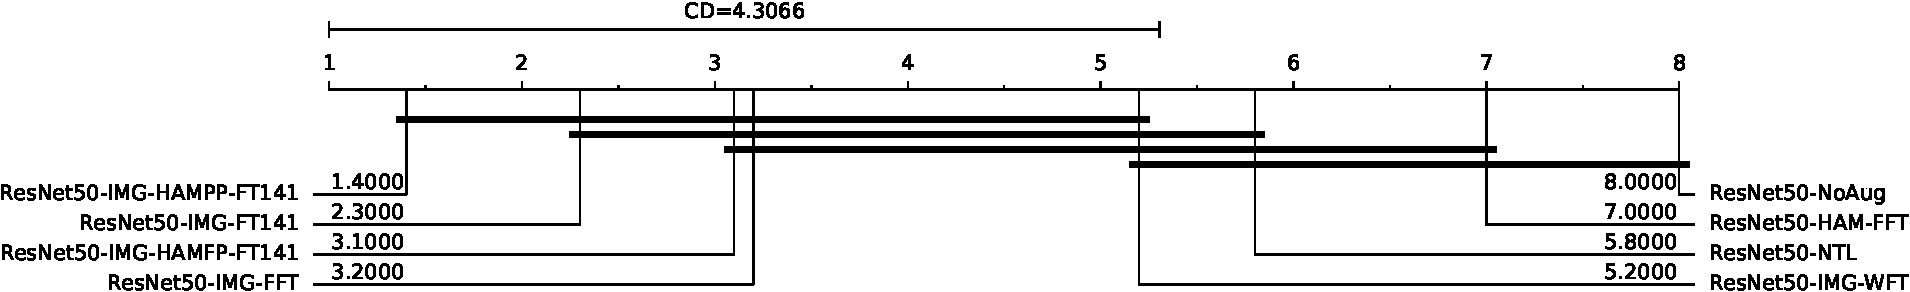
\includegraphics[width=\textwidth,keepaspectratio]{images/pretraining/CDRes-cropped.pdf}
	\caption[Accuracy critical difference diagram for ResNet50 based configurations]{Accuracy critical difference diagram for ResNet50 based configurations. The models are ordered by best to worst average ranking from left to right. The number beside a model’s name represents the average rank of the model. CD is the critical difference for Nemenyi post-hoc test. Thick horizontal line connects the models that are not statistically significantly different.}
	\label{fig:CD_ResNet}
\end{figure}

In the literature on recognizing EM from images, Čuk et al. \cite{Cuk2014} reported accuracies in the range of 69.23\% to 80.42\% using classical machine learning methods, and Burlina et al. \cite{Burlina2020} reported the best accuracy of 81.51\% using ResNet50 architecture for the case of EM vs all classification problems.
There was a common subset of images collected from the internet in both the dataset of Burlina et al. \cite{Burlina2018} and our Lyme dataset. ResNet50-Burlina model gave an accuracy of  76.05\% when tested on our full dataset as shown in Table \ref{tab:ResNet50-burlina-results}.
\begin{table}[tbh!]
	\centering
	\caption[Performance metrics of ResNet50-Burlina model trained by Burlina et al. \cite{Burlina2018} tested on the whole dataset of this study]{Performance metrics of ResNet50-Burlina model trained by Burlina et al. \cite{Burlina2018} tested on the whole dataset of this study. Within each cell, the value after $\pm$ symbol represents the standard deviation across five folds. Bold indicates the best result for each of the metrics.}
	\label{tab:ResNet50-burlina-results}
	\resizebox{\textwidth}{!}{%
		\begin{tabular}{llllllllllll}
			\toprule
			& \multicolumn{11}{c}{\textbf{Metric}}    \\ \cmidrule(l){2-12} 
			\multicolumn{1}{c}{\textbf{Model}} & \rotatebox{45}{Accuracy} & \rotatebox{45}{Sensitivity} & \rotatebox{45}{Specificity} & \rotatebox{45}{Precision} & \rotatebox{45}{NPV} & \rotatebox{45}{MCC} & \rotatebox{45}{Kappa} & \rotatebox{45}{LR$+$} & \rotatebox{45}{LR$-$} & \rotatebox{45}{F1-Score} & \rotatebox{45}{AUC}  \\ \midrule
			\begin{tabular}[c]{@{}l@{}}ResNet50-\\Burlina\end{tabular} & \begin{tabular}[c]{@{}l@{}}76.05\\ $\pm$0.74\end{tabular}& \begin{tabular}[c]{@{}l@{}}70.05\\ $\pm$3.6\end{tabular}& \begin{tabular}[c]{@{}l@{}}82.51\\ $\pm$3.31\end{tabular}& \begin{tabular}[c]{@{}l@{}}81.29\\ $\pm$2.1\end{tabular}& \begin{tabular}[c]{@{}l@{}}72.04\\ $\pm$1.71\end{tabular}& \begin{tabular}[c]{@{}l@{}}0.5294\\ $\pm$0.0132\end{tabular}& \begin{tabular}[c]{@{}l@{}}0.5229\\ $\pm$0.0145\end{tabular}& \begin{tabular}[c]{@{}l@{}}4.1017\\ $\pm$0.5172\end{tabular}& \begin{tabular}[c]{@{}l@{}}0.362\\ $\pm$0.0309\end{tabular}& \begin{tabular}[c]{@{}l@{}}0.7515\\ $\pm$0.0137\end{tabular}& \begin{tabular}[c]{@{}l@{}}0.481\\ $\pm$0.0509\end{tabular} \\ 
			\bottomrule
		\end{tabular}%
	}
\end{table} 
Performance metrics for the best performing configuration of all the CNN architectures used in this study are shown in Table \ref{tab:CNN-results}. ResNet50-141 achieved the best accuracy of 84.42\%. Most of the models except MobileNetV2-62, MobileNetV3Small-182, and NASNetMobile-617 showed good AUC values of above 90\% and good sensitivity suggesting that these CNNs can be a good choice for building pre-scanners for Lyme disease. Figure \ref{fig:CD_SOTA} shows the CD diagram in terms of accuracy for these models. The Friedman test null hypothesis was rejected with a $p$ value of 0.09564. From the CD diagram, we can see that ResNet50- 141 achieved the best average ranking followed by VGG19-13 and DenseNet121-379 respectively. Xception and Inception-based architectures had a similar ranking. NasNetMobile-617 ranked worst among all the models. The accuracy of the models varied from 81.3\% to 84.42\% and there is no statistically significant difference in terms of accuracy metric among most of the trained models. Overall, ResNet50-141 performed better in terms of various metrics (5 out of 11) as highlighted in Table \ref{tab:CNN-results}. We kept the confusion matrix, ROC curve, and cross-validation fold-wise details of all the trained models in Appendix Section \ref{sec:app-supply-pretrain} to make the chapter concise and readable.
\begin{figure}[]
	\centering
	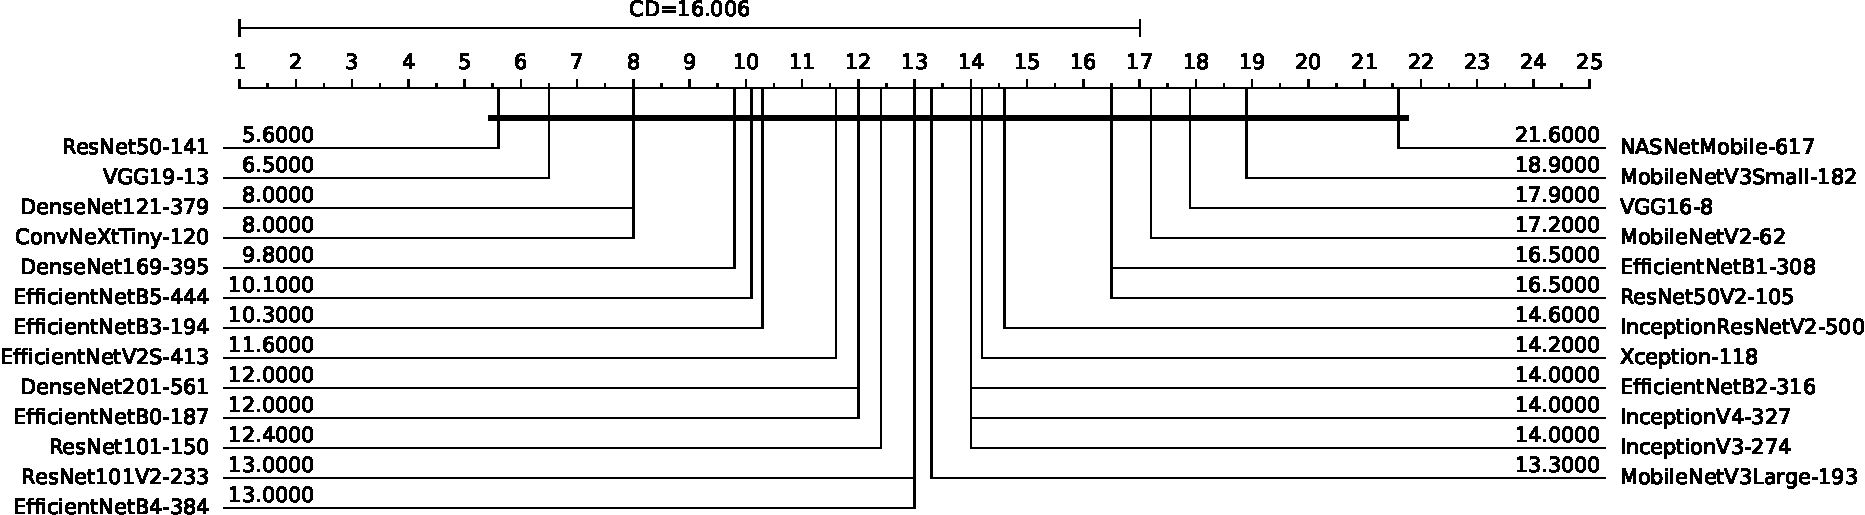
\includegraphics[width=\textwidth,keepaspectratio]{images/pretraining/CDAllSOTA-cropped.pdf}
	\caption[Accuracy critical difference diagram for the best performing configurations of the trained CNN models]{Accuracy critical difference diagram for the best performing configurations of the trained CNN models. The models are ordered by best to worst average ranking from left to right. The number beside a model’s name represents the average rank of the model. CD is the critical difference for Nemenyi post-hoc test. Thick horizontal line connects the models that are not statistically significantly different.}
	\label{fig:CD_SOTA}
\end{figure}

Table \ref{tab:complexity-table} summarizes the complexities of the CNN models used in this study.  The most lightweight model with the lowest number of parameters, FLOPs, and memory usage was MobileNetV3Small-182. InceptionResNetV2-500 has the highest number of parameters and memory usage and slowest inference time. Xception-118 was the fastest in terms of inference time. VGG19-13 required the highest number of FLOPs. ResNet50V2-105 required the least amount of time to train on average whereas, EfficientNetB5-444 was the slowest to train.

Table \ref{tab:gradcam} shows the Grad-CAM visualizations of the models trained on the same training fold for two test images. From the table, it can be seen that different versions of EfficientNet focused more on the lesion part of the image compared to other models. The squeeze-and-excitation \cite{Hu2020} channel attention used in EfficientNet can be the reason behind this behavior.

The experimental results showed that our proposed pre-training strategy utilizing dermoscopic dataset HAM10000 improved the performance of ImageNet pre-trained CNNs for recognizing clinical EM images. The results make it evident that CNNs have great potential to be used for Lyme disease pre-scanner application. Figure \ref{fig:bubble_chart} shows a bubble chart reporting model accuracy vs FLOPs. The size of each bubble represents the number of parameters of the model. This figure serves as a guideline for selecting models based on complexity and accuracy. It can be seen from the figure that EfficientNetB0-187 is a good choice with reasonable accuracy for resource-constrained mobile platforms. EfficientNetB0-187 also showed good results in Grad-CAM visualization. If resource constraint is not a problem, then RestNet50-141 can be used for the best accuracy.
\begin{figure}[h!]
	\centering
	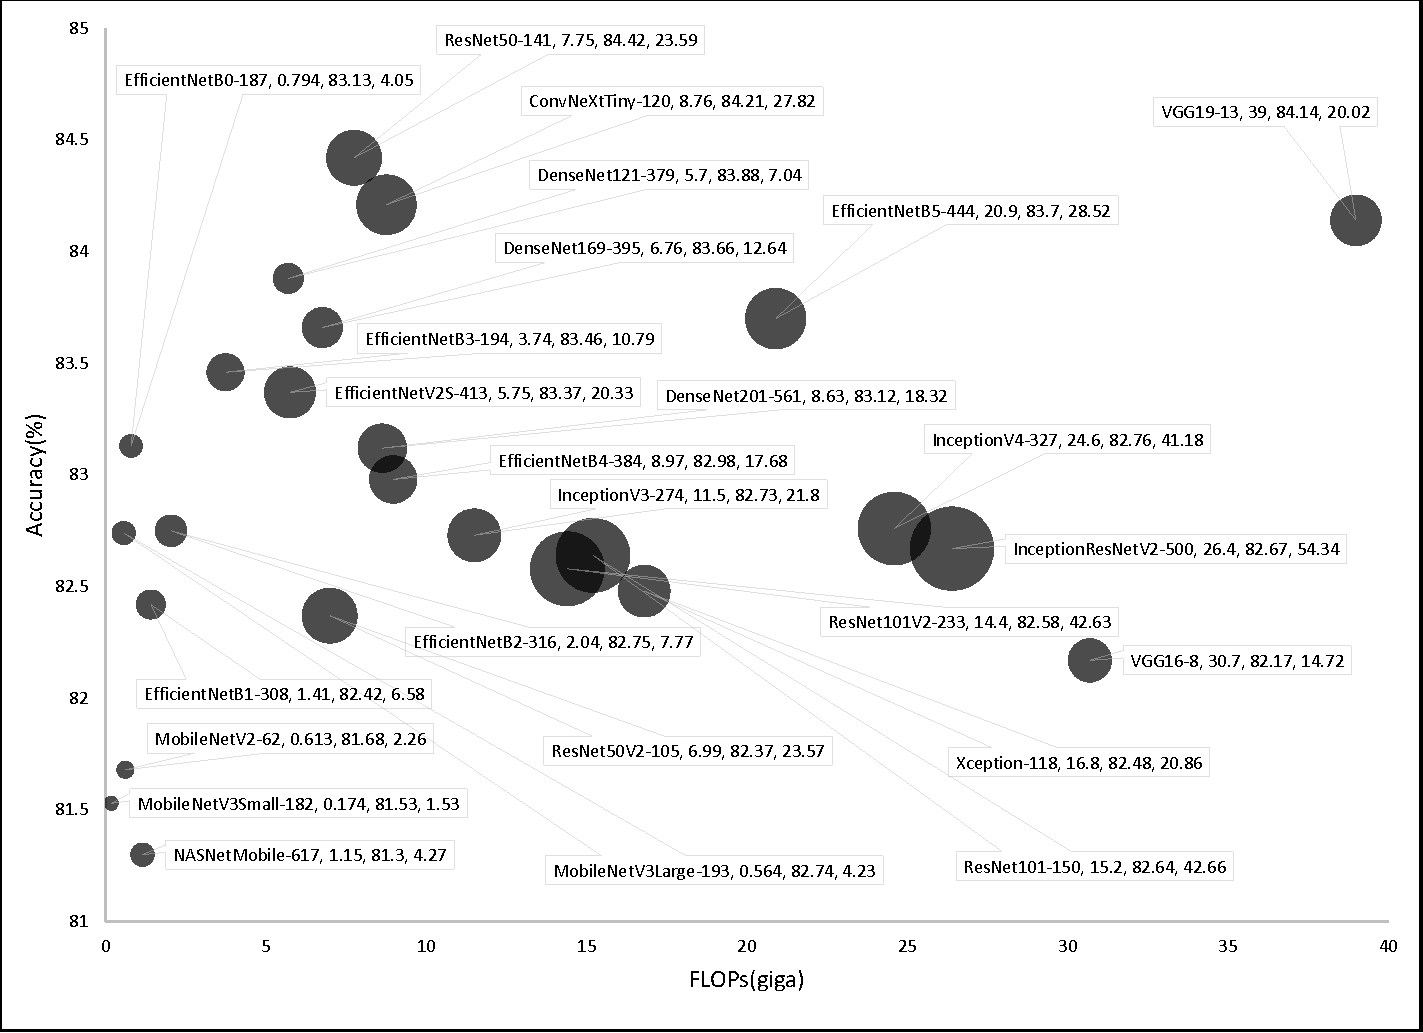
\includegraphics[width=\textwidth,keepaspectratio]{images/pretraining/bubble-chart-cropped.pdf}
	\caption[Bubble chart reporting model accuracy vs floating-point operations]{Bubble chart reporting model accuracy vs floating-point operations (FLOPs). The size of each bubble represents the number of model parameters measured in millions unit. Beside each model name the three values represent FLOPs, accuracy, and model parameters, respectively.}
	\label{fig:bubble_chart}
\end{figure}

Even the lightweight EfficientNetB0-187 model showed good performance, and it can be directly deployed in mobile devices without requiring an internet connection for processing the lesion image in a remote server. It can help people living in remote areas without good internet facilities with an initial assessment of the probability of Lyme disease. 

For this study, we utilized images from the internet alongside images collected from several hospitals in France. This approach was inspired by related studies on skin lesion analysis. 

Although a portion of images in our dataset was collected from the internet the annotation of the dataset is reliable because we ignored the online labels, and all the images were reannotated by expert dermatologists and infectiologists.

We made all the trained models publicly available, which can be utilized by others for transfer learning and building pre-scanners for Lyme disease. The trained CNN models are available at the link stated in Appendix Section \ref{sec:app-online-pretrain}.

%%%%%%%%%%%%%%%%%%%%%%%%%%%%%%%%%%%%%%%%%%%%%%%%%%%%%%%%%%%%%%%%%%%%%%%%
\section{Conclusion}\label{sec:concluion_pretrain}
%%%%%%%%%%%%%%%%%%%%%%%%%%%%%%%%%%%%%%%%%%%%%%%%%%%%%%%%%%%%%%%%%%%%%%%%
In this chapter, a pre-training strategy for improving clinical skin lesion image classification performance of ImageNet pre-trained convolutional neural networks by utilizing additional pre-training with dermoscopic images was proposed. We applied the strategy to benchmark twenty-five well-known CNNs based on predictive performance, complexity, significance tests, and heatmap visualization using a novel Lyme disease dataset to find out the effectiveness of CNNs for Lyme disease diagnosis from EM images. We also provided guidelines for model selection. We found that even the lightweight models like EffiicentNetB0 performed well suggesting the application of CNNs for Lyme disease pre-scanner mobile applications which can help people with an initial assessment of the probability of Lyme disease and referring them to expert dermatologist for further diagnosis. Resource intensive models like ResNet50 can be effective for building computer applications to assist non-expert practitioners with identifying EM.


\begin{tcolorbox}[enhanced,attach boxed title to top center={yshift=-3mm,yshifttext=-1mm},
	coltitle=black, colback=blue!5!white,colframe=blue!75!black,colbacktitle=violet!50!white,
	title=Key Points (Chapter \ref{chap:Pretraining}),fonttitle=\bfseries,
	boxed title style={colframe=black} ]
	\begin{itemize}
		\item We proposed a pre-training strategy of fine-tuning some layers from the end of an ImageNet pre-trained CNN architecture using a dermoscopic dataset before training the model on a clinical skin lesion dataset.
		\item The proposed pre-training strategy seemed effective for increasing model performance based on experimentation using a novel Lyme disease dataset.
		\item We benchmarked several state-of-the-art CNN architectures on the novel Lyme dataset utilizing our pre-training strategy.
		\item Experimental results suggest that even lightweight CNNs can be effective for Lyme disease pre-scanner mobile applications.
	\end{itemize}
\end{tcolorbox}

%%%%%%%%%%%%%Complexity Table%%%%%%%%%%%%%%%
\begin{table}[h!]
	\centering
	\caption[Complexity metrics of trained CNN models]{Complexity metrics of trained CNN models. Bold indicates the best result for each of the metrics.}
	\label{tab:complexity-table}
	\resizebox{\textwidth}{!}{%
		\begin{tabular}{@{}lccccc@{}}
			\toprule
			\multicolumn{1}{c}{\textbf{Model}} &
			\multicolumn{1}{c}{\textbf{Parameters}} &
			\multicolumn{1}{c}{\textbf{FLOPs}} &
			\multicolumn{1}{c}{\textbf{Average training time}} &
			\multicolumn{1}{c}{\textbf{GPU usage}} &
			\multicolumn{1}{c}{\textbf{Average inference time}} \\
			&
			\multicolumn{1}{c}{(million)} &
			\multicolumn{1}{c}{(giga)} &
			\multicolumn{1}{c}{(sec per epoch)} &
			\multicolumn{1}{c}{(megabyte)} &
			\multicolumn{1}{c}{(sec per image)} \\ \midrule
			VGG16-8               & 14.72         & 30.7           & 111         & 565          & 0.0426 \\
			VGG19-13              & 20.02         & 39             & 164         & 565          & 0.0431 \\
			ResNet50-141          & 23.59         & 7.75           & 113         & 821          & 0.0484 \\
			ResNet101-150         & 42.66         & 15.2           & 123.33      & 821          & 0.0539 \\
			ResNet50V2-105        & 23.57         & 6.99           & 76          & 821          & 0.0464 \\
			ResNet101V2-233       & 42.63         & 14.4           & 152         & 821          & 0.0599 \\
			InceptionV3-274       & 21.8          & 11.5           & 133         & 821          & 0.054  \\
			InceptionV4-327       & 41.18         & 24.6           & 223.33      & 1333         & 0.0735 \\
			InceptionResNetV2-500 & 54.34         & 26.4           & 281.33      & 1333         & 0.0958 \\
			Xception-118          & 20.86         & 16.8           & 243.33      & 821          & 0.0392 \\
			DenseNet121-379       & 7.04          & 5.7            & 140.67      & 437          & 0.0673 \\
			DenseNet169-395       & 12.64         & 6.76           & 130         & 565          & 0.0686 \\
			DenseNet201-561       & 18.32         & 8.63           & 182.67      & 565          & 0.084  \\
			MobileNetV2-62        & 2.26          & 0.613          & 78          & \textbf{341} & 0.0429 \\
			MobileNetV3Small-182  & \textbf{1.53} & \textbf{0.174} & 81          & \textbf{341} & 0.0444 \\
			MobileNetV3Large-193  & 4.23          & 0.564          & 86.33       & 373          & 0.0444 \\
			NASNetMobile -617     & 4.27          & 1.15           & 152         & 373          & 0.0741 \\
			EfficientNetB0-187    & 4.05          & 0.794          & 87          & 373          & 0.0523 \\
			EfficientNetB1-308    & 6.58          & 1.41           & 158.33      & 437          & 0.0546 \\
			EfficientNetB2-316    & 7.77          & 2.04           & 210         & 437          & 0.0565 \\
			EfficientNetB3-194    & 10.79         & 3.74           & 143         & 565          & 0.0648 \\
			EfficientNetB4-384    & 17.68         & 8.97           & 431         & 565          & 0.0614 \\
			EfficientNetB5-444    & 28.52         & 20.9           & 771         & 821          & 0.0659 \\
			EfficientNetV2S-413   & 20.33         & 5.75           & \textbf{50} & 591          & 0.934  \\
			ConvNeXtTiny-120      & 27.82         & 8.76           & 95          & 847          & 0.0664 \\ \bottomrule
		\end{tabular}%
	}
\end{table}
%%%%%%%%%%%%%Complexity Table%%%%%%%%%%%%%%%

%%%%%%%%%%%%%BIG TABLE%%%%%%%%%%%%%%%%%%%
\begin{table}[]
	\centering
	\caption[Five-fold cross-validation performance metrics for the best performing configurations of the trained CNN models]{Five-fold cross-validation performance metrics for the best performing configurations of the trained CNN models. Within each cell, the value after (±) symbol represents the standard deviation across five folds. Bold indicates the best result for each of the metrics.}
	\label{tab:CNN-results}
	\resizebox{\textwidth}{!}{%
		\begin{tabular}{llllllllllll}
			\toprule
			& \multicolumn{11}{c}{\textbf{Metric}}    \\ \cmidrule(l){2-12} 
			\multicolumn{1}{c}{\textbf{Model}} & \rotatebox{45}{Accuracy} & \rotatebox{45}{Sensitivity} & \rotatebox{45}{Specificity} & \rotatebox{45}{Precision} & \rotatebox{45}{NPV} & \rotatebox{45}{MCC} & \rotatebox{45}{Kappa} & \rotatebox{45}{LR$+$} & \rotatebox{45}{LR$-$} & \rotatebox{45}{F1-Score} & \rotatebox{45}{AUC}  \\ \midrule
			VGG16-8 & \begin{tabular}[c]{@{}l@{}}82.17 \\ $\pm$ 1.23\end{tabular}& \begin{tabular}[c]{@{}l@{}}85.77 \\ $\pm$ 3.58\end{tabular}& \begin{tabular}[c]{@{}l@{}}78.31 \\ $\pm$ 4.36\end{tabular}& \begin{tabular}[c]{@{}l@{}}81.12 \\ $\pm$ 2.62\end{tabular}& \begin{tabular}[c]{@{}l@{}}83.88 \\ $\pm$ 3.02\end{tabular}& \begin{tabular}[c]{@{}l@{}}0.6453 \\ $\pm$ 0.0253\end{tabular}& \begin{tabular}[c]{@{}l@{}}0.6422 \\ $\pm$ 0.0249\end{tabular}& \begin{tabular}[c]{@{}l@{}}4.0983 \\ $\pm$ 0.7329\end{tabular}& \begin{tabular}[c]{@{}l@{}}0.1802 \\ $\pm$ 0.0388\end{tabular}& \begin{tabular}[c]{@{}l@{}}0.8328 \\ $\pm$ 0.0116\end{tabular}& \begin{tabular}[c]{@{}l@{}}0.9011 \\ $\pm$ 0.0079\end{tabular}\\
			\cmidrule(lr){1-12}
			
			VGG19-13 & \begin{tabular}[c]{@{}l@{}}84.14 \\ $\pm$ 1.62\end{tabular}& \begin{tabular}[c]{@{}l@{}}85.29 \\ $\pm$ 1.69\end{tabular}& \begin{tabular}[c]{@{}l@{}}82.9 \\ $\pm$ 2.63\end{tabular}& \begin{tabular}[c]{@{}l@{}}\textbf{84.32} \\ $\pm$ 1.97\end{tabular}& \begin{tabular}[c]{@{}l@{}}84.0 \\ $\pm$ 1.67\end{tabular}& \begin{tabular}[c]{@{}l@{}}0.6826 \\ $\pm$ 0.0323\end{tabular}& \begin{tabular}[c]{@{}l@{}}0.6823 \\ $\pm$ 0.0326\end{tabular}& \begin{tabular}[c]{@{}l@{}}5.0924 \\ $\pm$ 0.6884\end{tabular}& \begin{tabular}[c]{@{}l@{}}0.1777 \\ $\pm$ 0.0214\end{tabular}& \begin{tabular}[c]{@{}l@{}}0.8479 \\ $\pm$ 0.0146\end{tabular}& \begin{tabular}[c]{@{}l@{}}0.913 \\ $\pm$ 0.0074\end{tabular}\\ 
			\cmidrule(lr){1-12}
			
			ResNet50-141 & \begin{tabular}[c]{@{}l@{}}\textbf{84.42} \\ $\pm$ 1.36\end{tabular}& \begin{tabular}[c]{@{}l@{}}87.93 \\ $\pm$ 1.47\end{tabular}& \begin{tabular}[c]{@{}l@{}}80.65 \\ $\pm$ 3.59\end{tabular}& \begin{tabular}[c]{@{}l@{}}83.1 \\ $\pm$ 2.49\end{tabular}& \begin{tabular}[c]{@{}l@{}}86.19 \\ $\pm$ 1.27\end{tabular}& \begin{tabular}[c]{@{}l@{}}\textbf{0.6893} \\ $\pm$ 0.0263\end{tabular}& \begin{tabular}[c]{@{}l@{}}\textbf{0.6874} \\ $\pm$ 0.0277\end{tabular}& \begin{tabular}[c]{@{}l@{}}4.703 \\ $\pm$ 0.8624\end{tabular}& \begin{tabular}[c]{@{}l@{}}0.1493 \\ $\pm$ 0.0155\end{tabular}& \begin{tabular}[c]{@{}l@{}}\textbf{0.8541} \\ $\pm$ 0.0106\end{tabular}& \begin{tabular}[c]{@{}l@{}}\textbf{0.9189} \\ $\pm$ 0.0115\end{tabular}\\ 
			\cmidrule(lr){1-12}
			
			\begin{tabular}[c]{@{}l@{}}ResNet50V2-\\105\end{tabular} & \begin{tabular}[c]{@{}l@{}}82.37 \\ $\pm$ 2.15\end{tabular}& \begin{tabular}[c]{@{}l@{}}85.53 \\ $\pm$ 3.35\end{tabular}& \begin{tabular}[c]{@{}l@{}}78.96 \\ $\pm$ 6.13\end{tabular}& \begin{tabular}[c]{@{}l@{}}81.66 \\ $\pm$ 3.83\end{tabular}& \begin{tabular}[c]{@{}l@{}}83.72 \\ $\pm$ 2.63\end{tabular}& \begin{tabular}[c]{@{}l@{}}0.6493 \\ $\pm$ 0.0411\end{tabular}& \begin{tabular}[c]{@{}l@{}}0.6461 \\ $\pm$ 0.0439\end{tabular}& \begin{tabular}[c]{@{}l@{}}4.3618 \\ $\pm$ 1.0495\end{tabular}& \begin{tabular}[c]{@{}l@{}}0.1819 \\ $\pm$ 0.0349\end{tabular}& \begin{tabular}[c]{@{}l@{}}0.8343 \\ $\pm$ 0.017\end{tabular}& \begin{tabular}[c]{@{}l@{}}0.9013 \\ $\pm$ 0.0133\end{tabular}\\ 
			\cmidrule(lr){1-12}
			
			\begin{tabular}[c]{@{}l@{}}ResNet101V2-\\233\end{tabular} & \begin{tabular}[c]{@{}l@{}}82.58 \\ $\pm$ 2.21\end{tabular}& \begin{tabular}[c]{@{}l@{}}81.9 \\ $\pm$ 4.78\end{tabular}& \begin{tabular}[c]{@{}l@{}}\textbf{83.32} \\ $\pm$ 3.71\end{tabular}& \begin{tabular}[c]{@{}l@{}}84.17 \\ $\pm$ 2.55\end{tabular}& \begin{tabular}[c]{@{}l@{}}81.31 \\ $\pm$ 3.7\end{tabular}& \begin{tabular}[c]{@{}l@{}}0.6535 \\ $\pm$ 0.0429\end{tabular}& \begin{tabular}[c]{@{}l@{}}0.6515 \\ $\pm$ 0.0439\end{tabular}& \begin{tabular}[c]{@{}l@{}}\textbf{5.104} \\ $\pm$ 0.9811\end{tabular}& \begin{tabular}[c]{@{}l@{}}0.2163 \\ $\pm$ 0.0541\end{tabular}& \begin{tabular}[c]{@{}l@{}}0.8292 \\ $\pm$ 0.0254\end{tabular}& \begin{tabular}[c]{@{}l@{}}0.9118 \\ $\pm$ 0.0149\end{tabular}\\ 
			\cmidrule(lr){1-12}
			
			\begin{tabular}[c]{@{}l@{}}InceptionV3-\\274\end{tabular} & \begin{tabular}[c]{@{}l@{}}82.73 \\ $\pm$ 2.08\end{tabular}& \begin{tabular}[c]{@{}l@{}}86.57 \\ $\pm$ 2.42\end{tabular}& \begin{tabular}[c]{@{}l@{}}78.6 \\ $\pm$ 2.8\end{tabular}& \begin{tabular}[c]{@{}l@{}}81.33 \\ $\pm$ 2.12\end{tabular}& \begin{tabular}[c]{@{}l@{}}84.52 \\ $\pm$ 2.52\end{tabular}& \begin{tabular}[c]{@{}l@{}}0.6551 \\ $\pm$ 0.0419\end{tabular}& \begin{tabular}[c]{@{}l@{}}0.6533 \\ $\pm$ 0.0419\end{tabular}& \begin{tabular}[c]{@{}l@{}}4.1259 \\ $\pm$ 0.639\end{tabular}& \begin{tabular}[c]{@{}l@{}}0.1714 \\ $\pm$ 0.0328\end{tabular}& \begin{tabular}[c]{@{}l@{}}0.8385 \\ $\pm$ 0.0195\end{tabular}& \begin{tabular}[c]{@{}l@{}}0.9052 \\ $\pm$ 0.0185\end{tabular}\\ 
			
			\cmidrule(lr){1-12}
			
			\begin{tabular}[c]{@{}l@{}}InceptionV4-\\327\end{tabular} & \begin{tabular}[c]{@{}l@{}}82.76 \\ $\pm$ 1.78\end{tabular}& \begin{tabular}[c]{@{}l@{}}85.7 \\ $\pm$ 3.96\end{tabular}& \begin{tabular}[c]{@{}l@{}}79.58 \\ $\pm$ 2.87\end{tabular}& \begin{tabular}[c]{@{}l@{}}81.92 \\ $\pm$ 1.8\end{tabular}& \begin{tabular}[c]{@{}l@{}}84.02 \\ $\pm$ 3.41\end{tabular}& \begin{tabular}[c]{@{}l@{}}0.6561 \\ $\pm$ 0.0358\end{tabular}& \begin{tabular}[c]{@{}l@{}}0.6541 \\ $\pm$ 0.0353\end{tabular}& \begin{tabular}[c]{@{}l@{}}4.2716 \\ $\pm$ 0.5734\end{tabular}& \begin{tabular}[c]{@{}l@{}}0.179 \\ $\pm$ 0.0465\end{tabular}& \begin{tabular}[c]{@{}l@{}}0.837 \\ $\pm$ 0.0197\end{tabular}& \begin{tabular}[c]{@{}l@{}}0.9092 \\ $\pm$ 0.019\end{tabular}\\ 
			
			\cmidrule(lr){1-12}
			
			\begin{tabular}[c]{@{}l@{}}Inception\\ResNetV2-500\end{tabular} & \begin{tabular}[c]{@{}l@{}}82.67\\ $\pm$2.06\end{tabular}& \begin{tabular}[c]{@{}l@{}}83.54\\ $\pm$3.88\end{tabular}& \begin{tabular}[c]{@{}l@{}}81.74\\ $\pm$3.16\end{tabular}& \begin{tabular}[c]{@{}l@{}}83.17\\ $\pm$2.16\end{tabular}& \begin{tabular}[c]{@{}l@{}}82.37\\ $\pm$3.32\end{tabular}& \begin{tabular}[c]{@{}l@{}}0.6541\\ $\pm$0.0406\end{tabular}& \begin{tabular}[c]{@{}l@{}}0.653\\ $\pm$0.041\end{tabular}& \begin{tabular}[c]{@{}l@{}}4.6886\\ $\pm$0.7264\end{tabular}& \begin{tabular}[c]{@{}l@{}}0.2009\\ $\pm$0.0456\end{tabular}& \begin{tabular}[c]{@{}l@{}}0.8329\\ $\pm$0.0218\end{tabular}& \begin{tabular}[c]{@{}l@{}}0.9011\\ $\pm$0.0133\end{tabular}\\ 
			
			\cmidrule(lr){1-12}
			
			Xception-118 & \begin{tabular}[c]{@{}l@{}}82.48\\ $\pm$2.45\end{tabular}& \begin{tabular}[c]{@{}l@{}}83.16\\ $\pm$5.1\end{tabular}& \begin{tabular}[c]{@{}l@{}}81.75\\ $\pm$2.76\end{tabular}& \begin{tabular}[c]{@{}l@{}}83.08\\ $\pm$1.94\end{tabular}& \begin{tabular}[c]{@{}l@{}}82.16\\ $\pm$4.4\end{tabular}& \begin{tabular}[c]{@{}l@{}}0.6507\\ $\pm$0.0487\end{tabular}& \begin{tabular}[c]{@{}l@{}}0.6492\\ $\pm$0.0484\end{tabular}& \begin{tabular}[c]{@{}l@{}}4.6434\\ $\pm$0.6571\end{tabular}& \begin{tabular}[c]{@{}l@{}}0.2054\\ $\pm$0.0609\end{tabular}& \begin{tabular}[c]{@{}l@{}}0.8304\\ $\pm$0.0276\end{tabular}& \begin{tabular}[c]{@{}l@{}}0.9081\\ $\pm$0.0148\end{tabular}\\ 
			
			\cmidrule(lr){1-12}
			
			\begin{tabular}[c]{@{}l@{}}DenseNet121-\\379\end{tabular} & \begin{tabular}[c]{@{}l@{}}83.88\\ $\pm$0.92\end{tabular}& \begin{tabular}[c]{@{}l@{}}85.85\\ $\pm$1.76\end{tabular}& \begin{tabular}[c]{@{}l@{}}81.75\\ $\pm$0.95\end{tabular}& \begin{tabular}[c]{@{}l@{}}83.49\\ $\pm$0.69\end{tabular}& \begin{tabular}[c]{@{}l@{}}84.35\\ $\pm$1.57\end{tabular}& \begin{tabular}[c]{@{}l@{}}0.6773\\ $\pm$0.0186\end{tabular}& \begin{tabular}[c]{@{}l@{}}0.6768\\ $\pm$0.0184\end{tabular}& \begin{tabular}[c]{@{}l@{}}4.7169\\ $\pm$0.254\end{tabular}& \begin{tabular}[c]{@{}l@{}}0.173\\ $\pm$0.0211\end{tabular}& \begin{tabular}[c]{@{}l@{}}0.8465\\ $\pm$0.01\end{tabular}& \begin{tabular}[c]{@{}l@{}}0.9158\\ $\pm$0.0097\end{tabular}\\ 
			
			\cmidrule(lr){1-12}
			
			\begin{tabular}[c]{@{}l@{}}DenseNet169-\\395\end{tabular} & \begin{tabular}[c]{@{}l@{}}83.66\\ $\pm$1.25\end{tabular}& \begin{tabular}[c]{@{}l@{}}\textbf{88.6}\\ $\pm$3.59\end{tabular}& \begin{tabular}[c]{@{}l@{}}78.35\\ $\pm$2.75\end{tabular}& \begin{tabular}[c]{@{}l@{}}81.54\\ $\pm$1.53\end{tabular}& \begin{tabular}[c]{@{}l@{}}\textbf{86.68}\\ $\pm$3.33\end{tabular}& \begin{tabular}[c]{@{}l@{}}0.6758\\ $\pm$0.0265\end{tabular}& \begin{tabular}[c]{@{}l@{}}0.6717\\ $\pm$0.0249\end{tabular}& \begin{tabular}[c]{@{}l@{}}4.1454\\ $\pm$0.4187\end{tabular}& \begin{tabular}[c]{@{}l@{}}\textbf{0.1446}\\ $\pm$0.0414\end{tabular}& \begin{tabular}[c]{@{}l@{}}0.8486\\ $\pm$0.0138\end{tabular}& \begin{tabular}[c]{@{}l@{}}0.9123\\ $\pm$0.0129\end{tabular}\\ 
			
			\cmidrule(lr){1-12}
			
			\begin{tabular}[c]{@{}l@{}}DenseNet201-\\561\end{tabular} & \begin{tabular}[c]{@{}l@{}}83.12\\ $\pm$1.11\end{tabular}& \begin{tabular}[c]{@{}l@{}}85.61\\ $\pm$1.81\end{tabular}& \begin{tabular}[c]{@{}l@{}}80.45\\ $\pm$3.92\end{tabular}& \begin{tabular}[c]{@{}l@{}}82.61\\ $\pm$2.7\end{tabular}& \begin{tabular}[c]{@{}l@{}}83.93\\ $\pm$1.13\end{tabular}& \begin{tabular}[c]{@{}l@{}}0.663\\ $\pm$0.0221\end{tabular}& \begin{tabular}[c]{@{}l@{}}0.6615\\ $\pm$0.0228\end{tabular}& \begin{tabular}[c]{@{}l@{}}4.5729\\ $\pm$0.9885\end{tabular}& \begin{tabular}[c]{@{}l@{}}0.1783\\ $\pm$0.0153\end{tabular}& \begin{tabular}[c]{@{}l@{}}0.8403\\ $\pm$0.0073\end{tabular}& \begin{tabular}[c]{@{}l@{}}0.9125\\ $\pm$0.0083\end{tabular}\\ 
			
			\cmidrule(lr){1-12}
			
			
			\begin{tabular}[c]{@{}l@{}}MobileNetV2-\\62\end{tabular} & \begin{tabular}[c]{@{}l@{}}81.68\\ $\pm$1.99\end{tabular}& \begin{tabular}[c]{@{}l@{}}81.94\\ $\pm$3.49\end{tabular}& \begin{tabular}[c]{@{}l@{}}81.39\\ $\pm$1.26\end{tabular}& \begin{tabular}[c]{@{}l@{}}82.55\\ $\pm$1.21\end{tabular}& \begin{tabular}[c]{@{}l@{}}80.85\\ $\pm$3.09\end{tabular}& \begin{tabular}[c]{@{}l@{}}0.6337\\ $\pm$0.0394\end{tabular}& \begin{tabular}[c]{@{}l@{}}0.6332\\ $\pm$0.0395\end{tabular}& \begin{tabular}[c]{@{}l@{}}4.4256\\ $\pm$0.3596\end{tabular}& \begin{tabular}[c]{@{}l@{}}0.222\\ $\pm$0.0441\end{tabular}& \begin{tabular}[c]{@{}l@{}}0.8222\\ $\pm$0.0218\end{tabular}& \begin{tabular}[c]{@{}l@{}}0.8933\\ $\pm$0.0135\end{tabular}\\ 
			
			\cmidrule(lr){1-12}
			
			\begin{tabular}[c]{@{}l@{}}MobileNetV3\\Small-182\end{tabular} & \begin{tabular}[c]{@{}l@{}}81.53\\ $\pm$1.98\end{tabular}& \begin{tabular}[c]{@{}l@{}}84.93\\ $\pm$3.29\end{tabular}& \begin{tabular}[c]{@{}l@{}}77.87\\ $\pm$3.89\end{tabular}& \begin{tabular}[c]{@{}l@{}}80.6\\ $\pm$2.55\end{tabular}& \begin{tabular}[c]{@{}l@{}}82.91\\ $\pm$2.85\end{tabular}& \begin{tabular}[c]{@{}l@{}}0.6315\\ $\pm$0.0398\end{tabular}& \begin{tabular}[c]{@{}l@{}}0.6294\\ $\pm$0.04\end{tabular}& \begin{tabular}[c]{@{}l@{}}3.9496\\ $\pm$0.6356\end{tabular}& \begin{tabular}[c]{@{}l@{}}0.1933\\ $\pm$0.0386\end{tabular}& \begin{tabular}[c]{@{}l@{}}0.8265\\ $\pm$0.0186\end{tabular}& \begin{tabular}[c]{@{}l@{}}0.896\\ $\pm$0.013\end{tabular}\\ 
			
			\cmidrule(lr){1-12}
			
			\begin{tabular}[c]{@{}l@{}}MobileNetV3\\Large-193\end{tabular} & \begin{tabular}[c]{@{}l@{}}82.74\\ $\pm$2.17\end{tabular}& \begin{tabular}[c]{@{}l@{}}83.69\\ $\pm$0.43\end{tabular}& \begin{tabular}[c]{@{}l@{}}81.71\\ $\pm$4.6\end{tabular}& \begin{tabular}[c]{@{}l@{}}83.26\\ $\pm$3.39\end{tabular}& \begin{tabular}[c]{@{}l@{}}82.3\\ $\pm$0.89\end{tabular}& \begin{tabular}[c]{@{}l@{}}0.6548\\ $\pm$0.0437\end{tabular}& \begin{tabular}[c]{@{}l@{}}0.6542\\ $\pm$0.0442\end{tabular}& \begin{tabular}[c]{@{}l@{}}4.8573\\ $\pm$1.1585\end{tabular}& \begin{tabular}[c]{@{}l@{}}0.2002\\ $\pm$0.0117\end{tabular}& \begin{tabular}[c]{@{}l@{}}0.8344\\ $\pm$0.017\end{tabular}& \begin{tabular}[c]{@{}l@{}}0.9034\\ $\pm$0.0094\end{tabular}\\ 
			
			\cmidrule(lr){1-12}
			
			\begin{tabular}[c]{@{}l@{}}NASNet\\Mobile-617\end{tabular} & \begin{tabular}[c]{@{}l@{}}81.3\\ $\pm$1.45\end{tabular}& \begin{tabular}[c]{@{}l@{}}83.2\\ $\pm$1.66\end{tabular}& \begin{tabular}[c]{@{}l@{}}79.25\\ $\pm$3.98\end{tabular}& \begin{tabular}[c]{@{}l@{}}81.29\\ $\pm$2.65\end{tabular}& \begin{tabular}[c]{@{}l@{}}81.48\\ $\pm$1.07\end{tabular}& \begin{tabular}[c]{@{}l@{}}0.6261\\ $\pm$0.0287\end{tabular}& \begin{tabular}[c]{@{}l@{}}0.6251\\ $\pm$0.0297\end{tabular}& \begin{tabular}[c]{@{}l@{}}4.1452\\ $\pm$0.7283\end{tabular}& \begin{tabular}[c]{@{}l@{}}0.2117\\ $\pm$0.0156\end{tabular}& \begin{tabular}[c]{@{}l@{}}0.8219\\ $\pm$0.0108\end{tabular}& \begin{tabular}[c]{@{}l@{}}0.8897\\ $\pm$0.0152\end{tabular}\\ 
			
			
			\cmidrule(lr){1-12}
			
			\begin{tabular}[c]{@{}l@{}}EfficientNet\\B0-187\end{tabular} & \begin{tabular}[c]{@{}l@{}}83.13\\ $\pm$1.2\end{tabular}& \begin{tabular}[c]{@{}l@{}}85.21\\ $\pm$3.91\end{tabular}& \begin{tabular}[c]{@{}l@{}}80.89\\ $\pm$2.95\end{tabular}& \begin{tabular}[c]{@{}l@{}}82.83\\ $\pm$1.75\end{tabular}& \begin{tabular}[c]{@{}l@{}}83.79\\ $\pm$3.19\end{tabular}& \begin{tabular}[c]{@{}l@{}}0.6636\\ $\pm$0.0244\end{tabular}& \begin{tabular}[c]{@{}l@{}}0.6618\\ $\pm$0.0237\end{tabular}& \begin{tabular}[c]{@{}l@{}}4.5522\\ $\pm$0.6116\end{tabular}& \begin{tabular}[c]{@{}l@{}}0.1817\\ $\pm$0.0427\end{tabular}& \begin{tabular}[c]{@{}l@{}}0.8392\\ $\pm$0.0147\end{tabular}& \begin{tabular}[c]{@{}l@{}}0.9094\\ $\pm$0.0129\end{tabular}\\ 
			
			\cmidrule(lr){1-12}
			
			\begin{tabular}[c]{@{}l@{}}EfficientNet\\B1-308\end{tabular} & \begin{tabular}[c]{@{}l@{}}82.42\\ $\pm$1.04\end{tabular}& \begin{tabular}[c]{@{}l@{}}85.85\\ $\pm$2.14\end{tabular}& \begin{tabular}[c]{@{}l@{}}78.71\\ $\pm$3.75\end{tabular}& \begin{tabular}[c]{@{}l@{}}81.37\\ $\pm$2.34\end{tabular}& \begin{tabular}[c]{@{}l@{}}83.9\\ $\pm$1.59\end{tabular}& \begin{tabular}[c]{@{}l@{}}0.6492\\ $\pm$0.0202\end{tabular}& \begin{tabular}[c]{@{}l@{}}0.647\\ $\pm$0.0214\end{tabular}& \begin{tabular}[c]{@{}l@{}}4.1494\\ $\pm$0.6707\end{tabular}& \begin{tabular}[c]{@{}l@{}}0.179\\ $\pm$0.0209\end{tabular}& \begin{tabular}[c]{@{}l@{}}0.835\\ $\pm$0.0074\end{tabular}& \begin{tabular}[c]{@{}l@{}}0.9088\\ $\pm$0.0134\end{tabular}\\ 
			
			
			\cmidrule(lr){1-12}
			
			\begin{tabular}[c]{@{}l@{}}EfficientNet\\B2-316\end{tabular} & \begin{tabular}[c]{@{}l@{}}82.75\\ $\pm$1.4\end{tabular}& \begin{tabular}[c]{@{}l@{}}84.95\\ $\pm$3.41\end{tabular}& \begin{tabular}[c]{@{}l@{}}80.39\\ $\pm$3.02\end{tabular}& \begin{tabular}[c]{@{}l@{}}82.39\\ $\pm$1.91\end{tabular}& \begin{tabular}[c]{@{}l@{}}83.4\\ $\pm$2.69\end{tabular}& \begin{tabular}[c]{@{}l@{}}0.6556\\ $\pm$0.0276\end{tabular}& \begin{tabular}[c]{@{}l@{}}0.6542\\ $\pm$0.0279\end{tabular}& \begin{tabular}[c]{@{}l@{}}4.4211\\ $\pm$0.6202\end{tabular}& \begin{tabular}[c]{@{}l@{}}0.1865\\ $\pm$0.0379\end{tabular}& \begin{tabular}[c]{@{}l@{}}0.8359\\ $\pm$0.0158\end{tabular}& \begin{tabular}[c]{@{}l@{}}0.9075\\ $\pm$0.0082\end{tabular}\\ 
			
			\cmidrule(lr){1-12}
			
			\begin{tabular}[c]{@{}l@{}}EfficientNet\\B3-194\end{tabular} & \begin{tabular}[c]{@{}l@{}}83.46\\ $\pm$0.87\end{tabular}& \begin{tabular}[c]{@{}l@{}}85.15\\ $\pm$4.28\end{tabular}& \begin{tabular}[c]{@{}l@{}}81.64\\ $\pm$2.9\end{tabular}& \begin{tabular}[c]{@{}l@{}}83.4\\ $\pm$1.6\end{tabular}& \begin{tabular}[c]{@{}l@{}}83.9\\ $\pm$3.14\end{tabular}& \begin{tabular}[c]{@{}l@{}}0.6704\\ $\pm$0.0157\end{tabular}& \begin{tabular}[c]{@{}l@{}}0.6685\\ $\pm$0.0167\end{tabular}& \begin{tabular}[c]{@{}l@{}}4.7361\\ $\pm$0.6283\end{tabular}& \begin{tabular}[c]{@{}l@{}}0.1803\\ $\pm$0.0443\end{tabular}& \begin{tabular}[c]{@{}l@{}}0.8416\\ $\pm$0.0144\end{tabular}& \begin{tabular}[c]{@{}l@{}}0.9163\\ $\pm$0.0074\end{tabular}\\ 
			
			\cmidrule(lr){1-12}
			
			\begin{tabular}[c]{@{}l@{}}EfficientNet\\B4-384\end{tabular} & \begin{tabular}[c]{@{}l@{}}82.98\\ $\pm$1.31\end{tabular}& \begin{tabular}[c]{@{}l@{}}87.55\\ $\pm$2.2\end{tabular}& \begin{tabular}[c]{@{}l@{}}78.06\\ $\pm$3.76\end{tabular}& \begin{tabular}[c]{@{}l@{}}81.2\\ $\pm$2.33\end{tabular}& \begin{tabular}[c]{@{}l@{}}85.46\\ $\pm$1.76\end{tabular}& \begin{tabular}[c]{@{}l@{}}0.6613\\ $\pm$0.0249\end{tabular}& \begin{tabular}[c]{@{}l@{}}0.6581\\ $\pm$0.0268\end{tabular}& \begin{tabular}[c]{@{}l@{}}4.0946\\ $\pm$0.6159\end{tabular}& \begin{tabular}[c]{@{}l@{}}0.1589\\ $\pm$0.0233\end{tabular}& \begin{tabular}[c]{@{}l@{}}0.842\\ $\pm$0.0107\end{tabular}& \begin{tabular}[c]{@{}l@{}}0.9138\\ $\pm$0.0074\end{tabular}\\ 
			
			\cmidrule(lr){1-12}
			
			\begin{tabular}[c]{@{}l@{}}EfficientNet\\B5-444\end{tabular} & \begin{tabular}[c]{@{}l@{}}83.7\\ $\pm$1.21\end{tabular}& \begin{tabular}[c]{@{}l@{}}86.85\\ $\pm$2.89\end{tabular}& \begin{tabular}[c]{@{}l@{}}80.32\\ $\pm$3.73\end{tabular}& \begin{tabular}[c]{@{}l@{}}82.71\\ $\pm$2.39\end{tabular}& \begin{tabular}[c]{@{}l@{}}85.17\\ $\pm$2.38\end{tabular}& \begin{tabular}[c]{@{}l@{}}0.6752\\ $\pm$0.024\end{tabular}& \begin{tabular}[c]{@{}l@{}}0.6729\\ $\pm$0.0245\end{tabular}& \begin{tabular}[c]{@{}l@{}}4.5562\\ $\pm$0.7645\end{tabular}& \begin{tabular}[c]{@{}l@{}}0.1629\\ $\pm$0.0303\end{tabular}& \begin{tabular}[c]{@{}l@{}}0.8466\\ $\pm$0.0108\end{tabular}& \begin{tabular}[c]{@{}l@{}}0.9138\\ $\pm$0.0161\end{tabular}\\ 
			
			\cmidrule(lr){1-12}
			
			\begin{tabular}[c]{@{}l@{}}EfficientNet\\V2S-413\end{tabular} & \begin{tabular}[c]{@{}l@{}}83.37\\ $\pm$2.26\end{tabular}& \begin{tabular}[c]{@{}l@{}}84.53\\ $\pm$3.11\end{tabular}& \begin{tabular}[c]{@{}l@{}}82.13\\ $\pm$4.05\end{tabular}& \begin{tabular}[c]{@{}l@{}}83.68\\ $\pm$3.02\end{tabular}& \begin{tabular}[c]{@{}l@{}}83.26\\ $\pm$2.76\end{tabular}& \begin{tabular}[c]{@{}l@{}}0.6679\\ $\pm$0.0451\end{tabular}& \begin{tabular}[c]{@{}l@{}}0.6669\\ $\pm$0.0453\end{tabular}& \begin{tabular}[c]{@{}l@{}}4.9859\\ $\pm$1.1671\end{tabular}& \begin{tabular}[c]{@{}l@{}}0.1884\\ $\pm$0.0365\end{tabular}& \begin{tabular}[c]{@{}l@{}}0.8404\\ $\pm$0.0212\end{tabular}& \begin{tabular}[c]{@{}l@{}}0.9144\\ $\pm$0.0145\end{tabular}\\ 
			\cmidrule(lr){1-12}
			
			
			\begin{tabular}[c]{@{}l@{}}ConvNeXt\\Tiny-120\end{tabular} & \begin{tabular}[c]{@{}l@{}}84.21\\ $\pm$2.07\end{tabular}& \begin{tabular}[c]{@{}l@{}}86.72\\ $\pm$3.5\end{tabular}& \begin{tabular}[c]{@{}l@{}}81.51\\ $\pm$2.0\end{tabular}& \begin{tabular}[c]{@{}l@{}}83.45\\ $\pm$1.6\end{tabular}& \begin{tabular}[c]{@{}l@{}}85.23\\ $\pm$3.31\end{tabular}& \begin{tabular}[c]{@{}l@{}}0.6845\\ $\pm$0.0418\end{tabular}& \begin{tabular}[c]{@{}l@{}}0.6834\\ $\pm$0.0412\end{tabular}& \begin{tabular}[c]{@{}l@{}}4.7452\\ $\pm$0.5401\end{tabular}& \begin{tabular}[c]{@{}l@{}}0.1631\\ $\pm$0.0436\end{tabular}& \begin{tabular}[c]{@{}l@{}}0.8502\\ $\pm$0.0215\end{tabular}& \begin{tabular}[c]{@{}l@{}}0.9183\\ $\pm$0.015\end{tabular}\\ 
			
			
			\bottomrule
		\end{tabular}%
	}
\end{table}
%%%%%%%%%%%%%BIG TABLE%%%%%%%%%%%%%%%%%%%

\begin{landscape}
	\begin{table}[]
		\centering
		\caption {Grad-CAM heatmap visualization of the trained models.}
		\label{tab:gradcam}
		\begin{tabular}{@{}c c c c c c c c c c@{}}
			\toprule
			\multicolumn{2}{c}{VGG16-8} & \multicolumn{2}{c}{VGG19-13} & \multicolumn{2}{c}{ResNet50-141} & \multicolumn{2}{c}{ResNet101-150} & \multicolumn{2}{c}{ResNet50V2-105}\\
			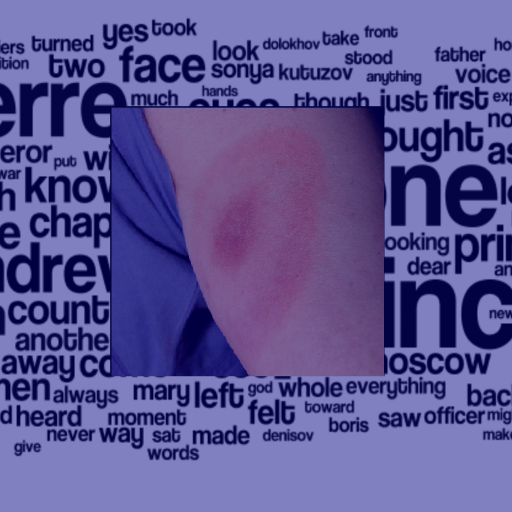
\includegraphics[width=.12\textheight ,keepaspectratio]{images/pretraining/gradcam/3/VGG16CombinedGradCam.png} &
			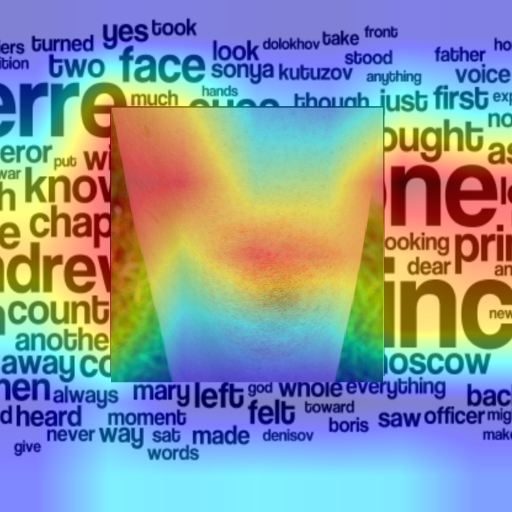
\includegraphics[width=.12\textheight ,keepaspectratio]{images/pretraining/gradcam/9/VGG16CombinedGradCam.png} &
			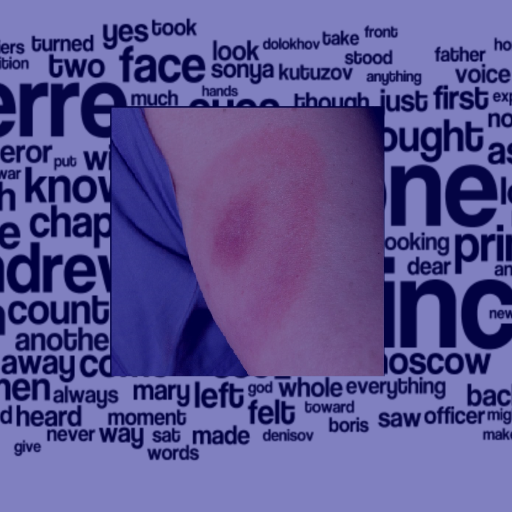
\includegraphics[width=.12\textheight ,keepaspectratio]{images/pretraining/gradcam/3/VGG19CombinedGradCam.png} &
			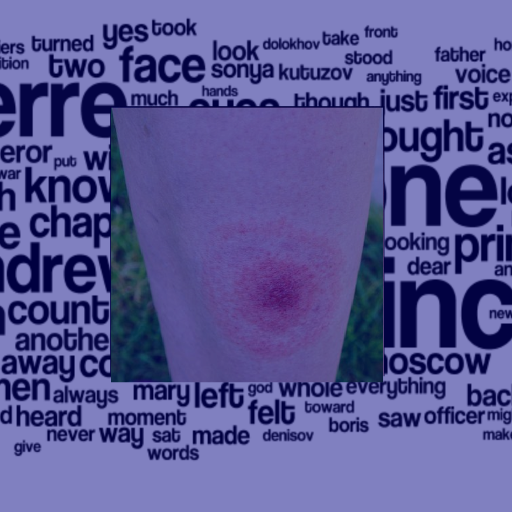
\includegraphics[width=.12\textheight ,keepaspectratio]{images/pretraining/gradcam/9/VGG19CombinedGradCam.png} &
			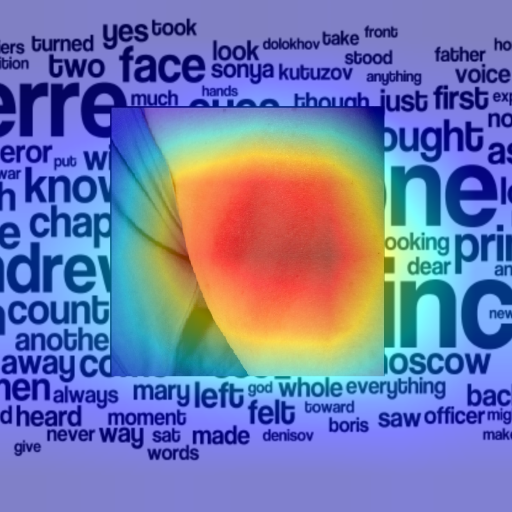
\includegraphics[width=.12\textheight ,keepaspectratio]{images/pretraining/gradcam/3/ResNet50CombinedGradCam.png} &
			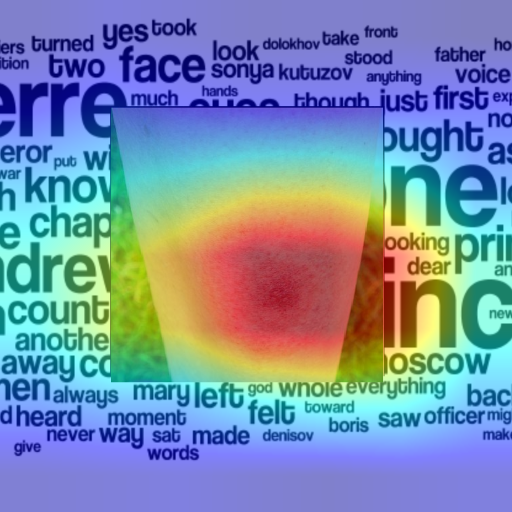
\includegraphics[width=.12\textheight ,keepaspectratio]{images/pretraining/gradcam/9/ResNet50CombinedGradCam.png} &
			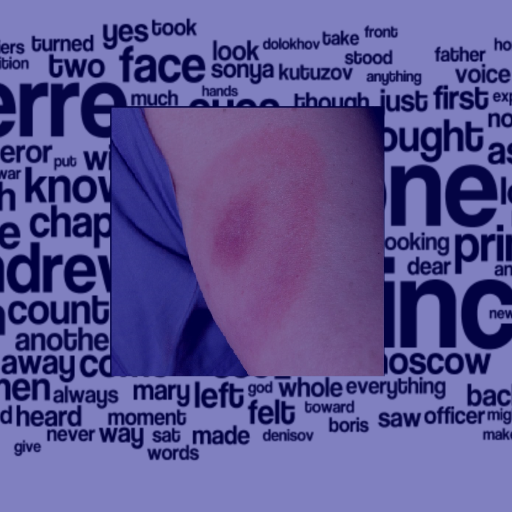
\includegraphics[width=.12\textheight ,keepaspectratio]{images/pretraining/gradcam/3/ResNet101CombinedGradCam.png} &
			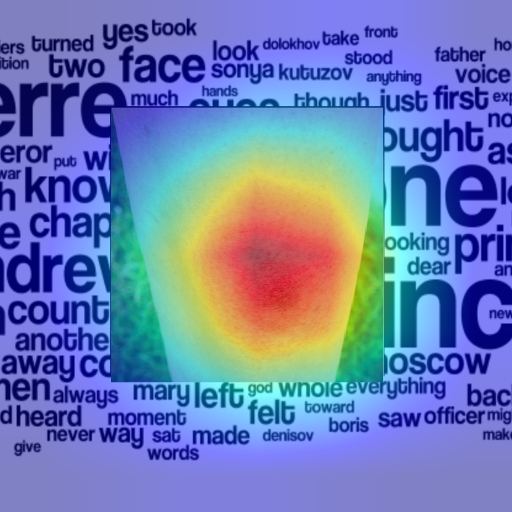
\includegraphics[width=.12\textheight ,keepaspectratio]{images/pretraining/gradcam/9/ResNet101CombinedGradCam.png} &
			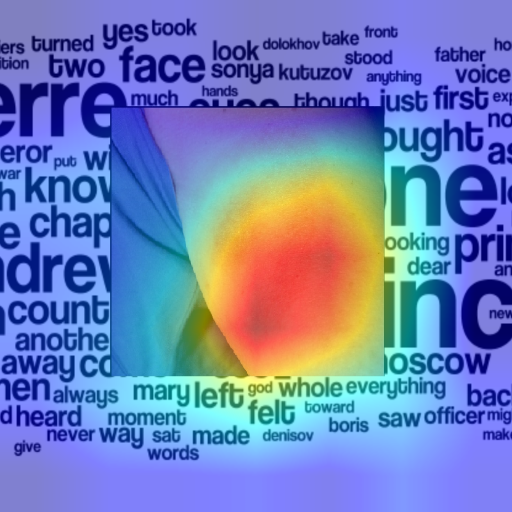
\includegraphics[width=.12\textheight ,keepaspectratio]{images/pretraining/gradcam/3/ResNet50V2CombinedGradCam.png} &
			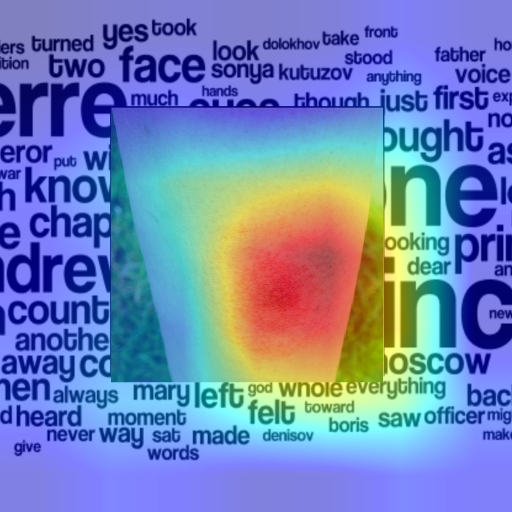
\includegraphics[width=.12\textheight ,keepaspectratio]{images/pretraining/gradcam/9/ResNet50V2CombinedGradCam.png}
			\\\cmidrule(lr){1-10}
			
			\multicolumn{2}{c}{ResNet101V2-233} & \multicolumn{2}{c}{InceptionV3-274} & \multicolumn{2}{c}{InceptionV4-327} & \multicolumn{2}{c}{InceptionResNetV2-500} & \multicolumn{2}{c}{Xception-118}\\
			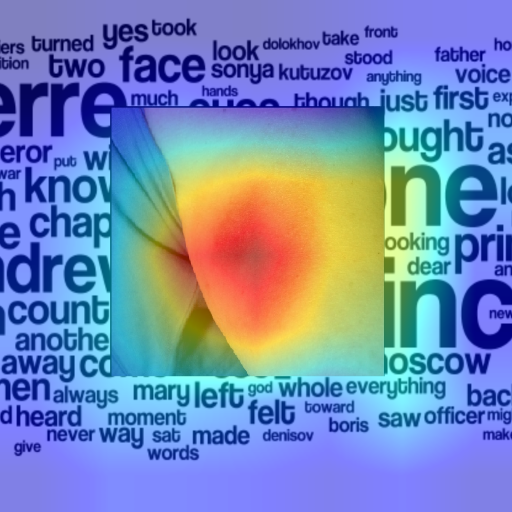
\includegraphics[width=.12\textheight ,keepaspectratio]{images/pretraining/gradcam/3/ResNet101V2CombinedGradCam.png} &
			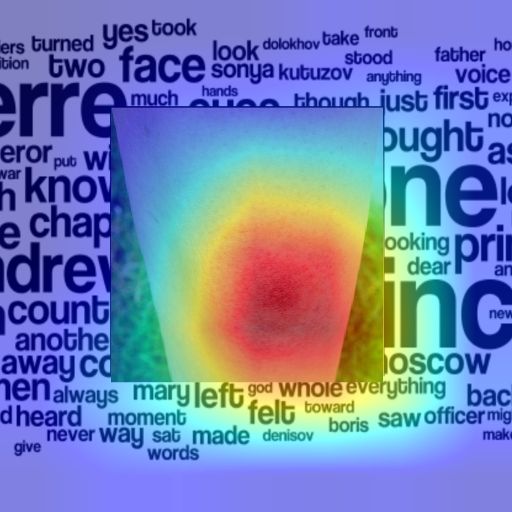
\includegraphics[width=.12\textheight ,keepaspectratio]{images/pretraining/gradcam/9/ResNet101V2CombinedGradCam.png} &
			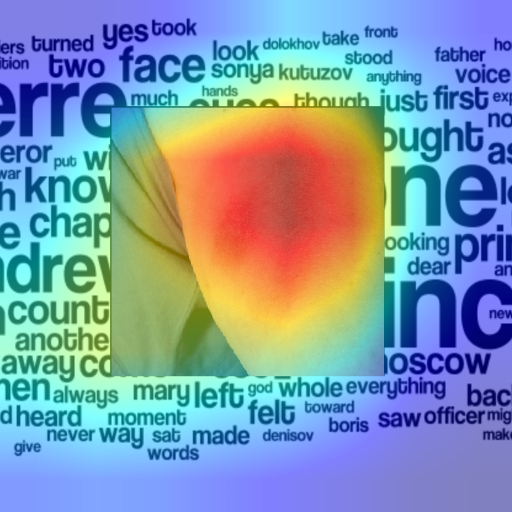
\includegraphics[width=.12\textheight ,keepaspectratio]{images/pretraining/gradcam/3/InceptionV3CombinedGradCam.png} &
			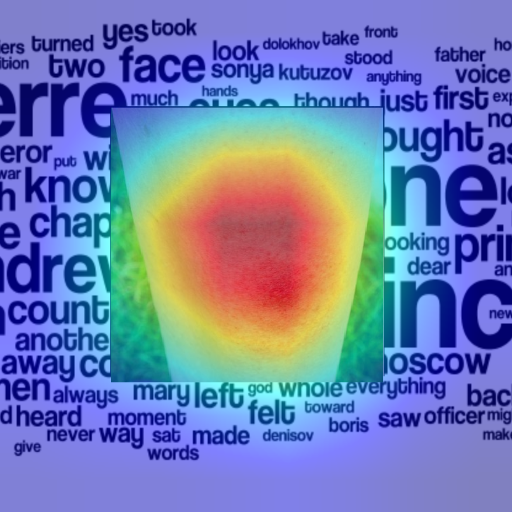
\includegraphics[width=.12\textheight ,keepaspectratio]{images/pretraining/gradcam/9/InceptionV3CombinedGradCam.png} &
			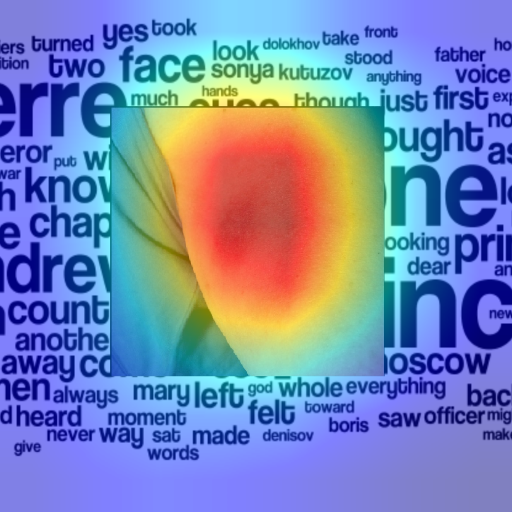
\includegraphics[width=.12\textheight ,keepaspectratio]{images/pretraining/gradcam/3/InceptionV4CombinedGradCam.png} &
			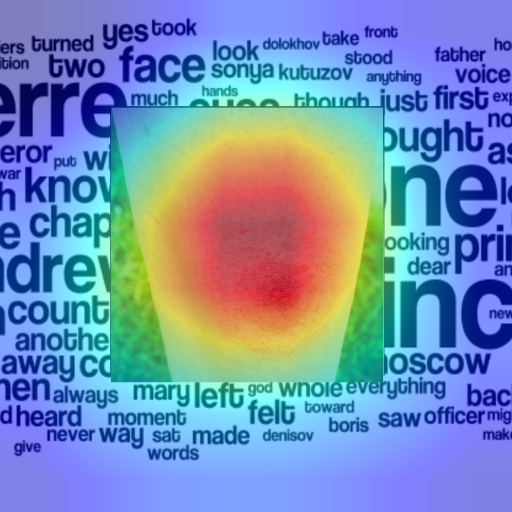
\includegraphics[width=.12\textheight ,keepaspectratio]{images/pretraining/gradcam/9/InceptionV4CombinedGradCam.png} &
			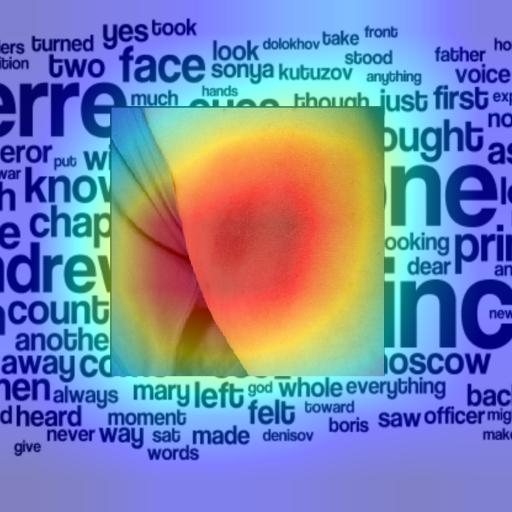
\includegraphics[width=.12\textheight ,keepaspectratio]{images/pretraining/gradcam/3/InceptionResNetV2CombinedGradCam.png} &
			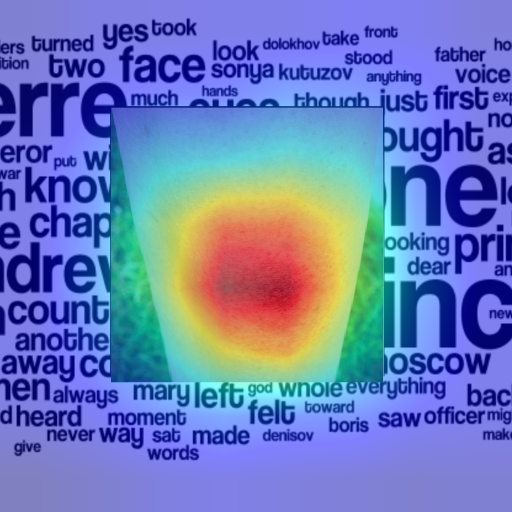
\includegraphics[width=.12\textheight ,keepaspectratio]{images/pretraining/gradcam/9/InceptionResNetV2CombinedGradCam.png} &
			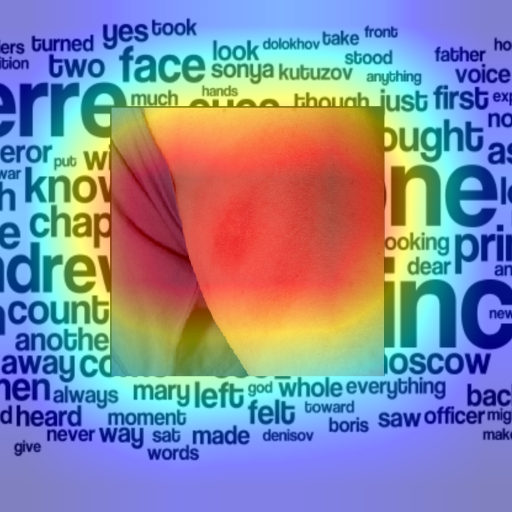
\includegraphics[width=.12\textheight ,keepaspectratio]{images/pretraining/gradcam/3/XceptionCombinedGradCam.png} &
			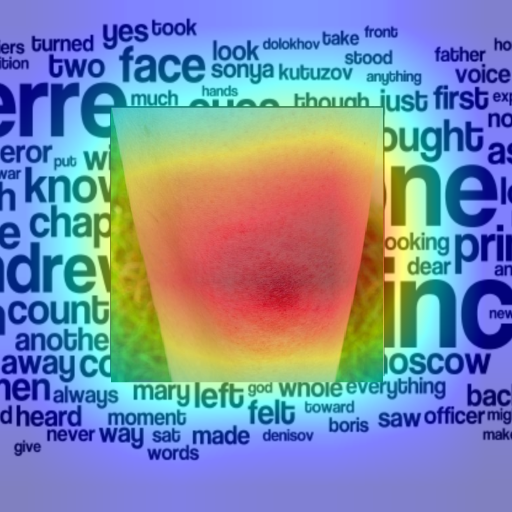
\includegraphics[width=.12\textheight ,keepaspectratio]{images/pretraining/gradcam/9/XceptionCombinedGradCam.png}
			\\\cmidrule(lr){1-10}
			
			\multicolumn{2}{c}{DenseNet121-379} & \multicolumn{2}{c}{DenseNet169-395} & \multicolumn{2}{c}{DenseNet201-561} & \multicolumn{2}{c}{MobileNetV2-62} & \multicolumn{2}{c}{MobileNetV3Small-182}\\
			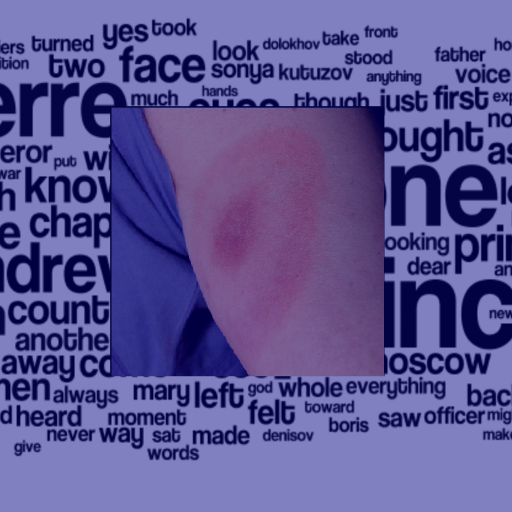
\includegraphics[width=.12\textheight ,keepaspectratio]{images/pretraining/gradcam/3/DenseNet121CombinedGradCam.png} &
			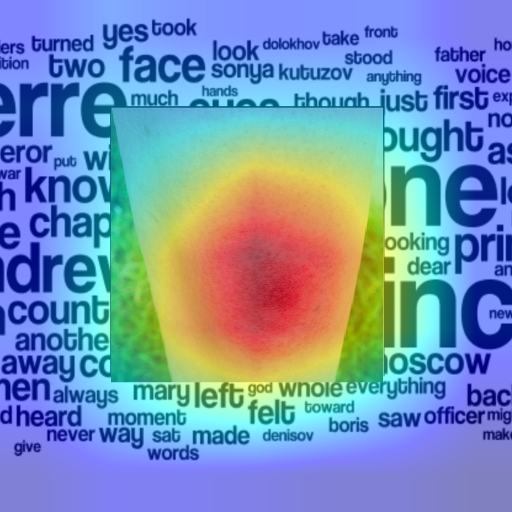
\includegraphics[width=.12\textheight ,keepaspectratio]{images/pretraining/gradcam/9/DenseNet121CombinedGradCam.png} &
			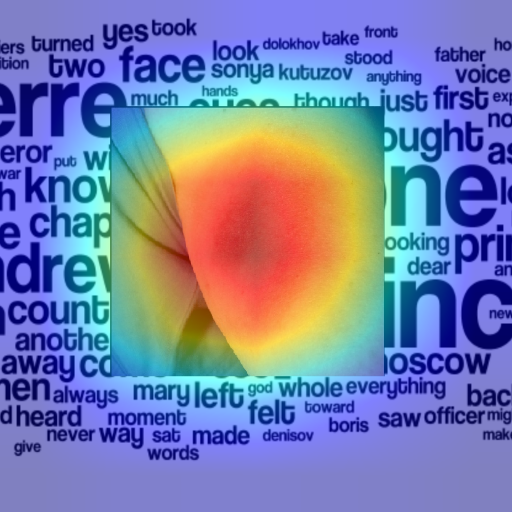
\includegraphics[width=.12\textheight ,keepaspectratio]{images/pretraining/gradcam/3/DenseNet169CombinedGradCam.png} &
			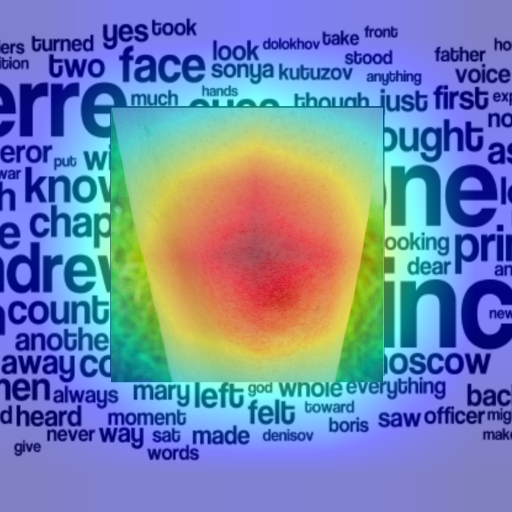
\includegraphics[width=.12\textheight ,keepaspectratio]{images/pretraining/gradcam/9/DenseNet169CombinedGradCam.png} &
			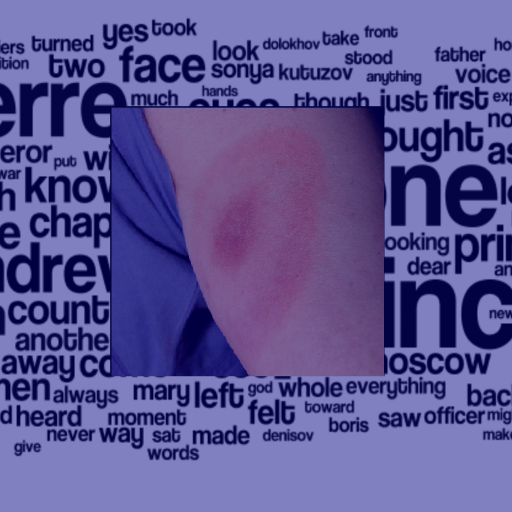
\includegraphics[width=.12\textheight ,keepaspectratio]{images/pretraining/gradcam/3/DenseNet201CombinedGradCam.png} &
			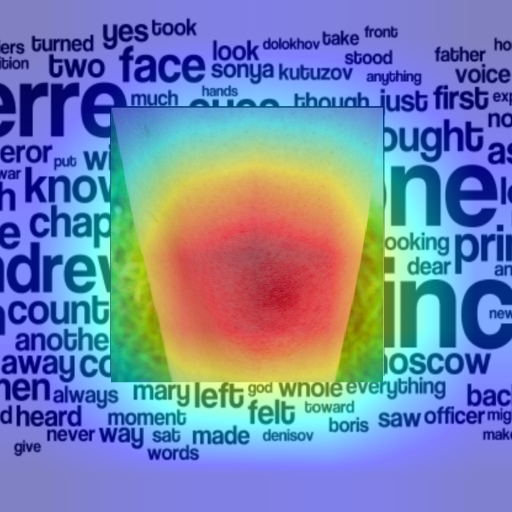
\includegraphics[width=.12\textheight ,keepaspectratio]{images/pretraining/gradcam/9/DenseNet201CombinedGradCam.png} &
			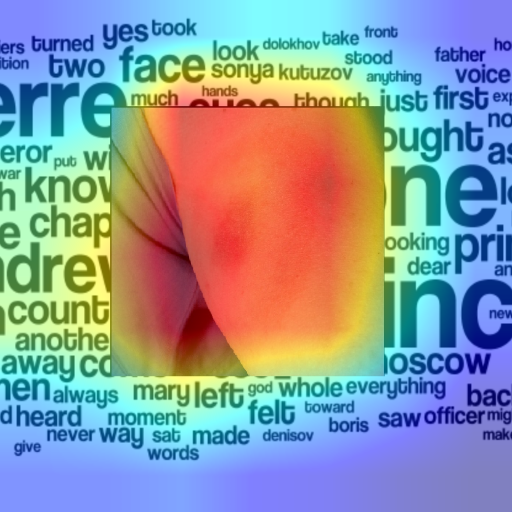
\includegraphics[width=.12\textheight ,keepaspectratio]{images/pretraining/gradcam/3/MobileNetV2CombinedGradCam.png} &
			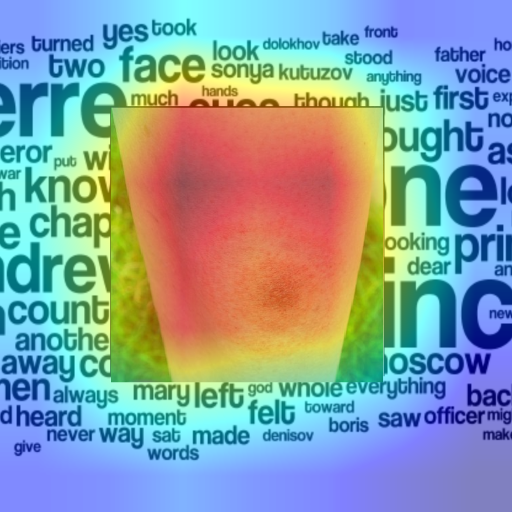
\includegraphics[width=.12\textheight ,keepaspectratio]{images/pretraining/gradcam/9/MobileNetV2CombinedGradCam.png} &
			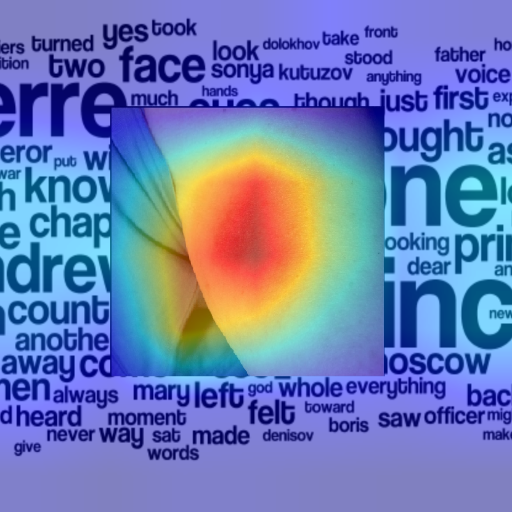
\includegraphics[width=.12\textheight ,keepaspectratio]{images/pretraining/gradcam/3/MobileNetV3SmallCombinedGradCam.png} &
			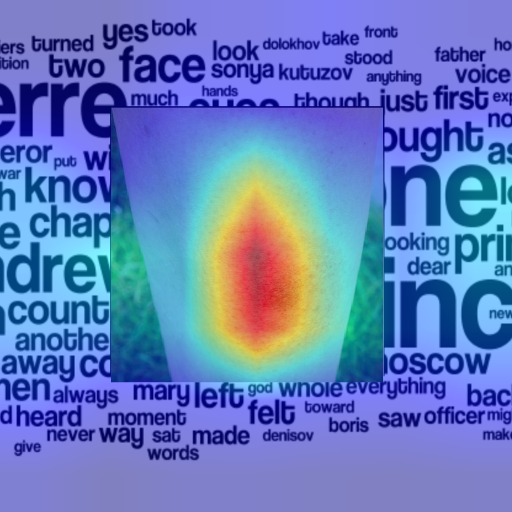
\includegraphics[width=.12\textheight ,keepaspectratio]{images/pretraining/gradcam/9/MobileNetV3SmallCombinedGradCam.png}
			\\\cmidrule(lr){1-10}
			
			\multicolumn{2}{c}{MobileNetV3Large-193} & \multicolumn{2}{c}{NASNetMobile-617} & \multicolumn{2}{c}{EfficientNetB0-187} & \multicolumn{2}{c}{EfficientNetB1-308} & \multicolumn{2}{c}{EfficientNetB2-316}\\
			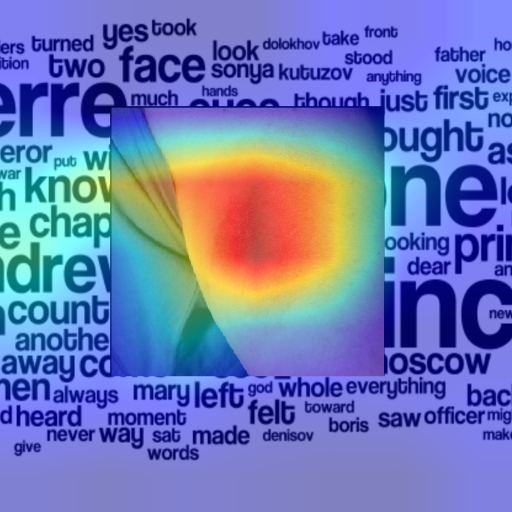
\includegraphics[width=.12\textheight ,keepaspectratio]{images/pretraining/gradcam/3/MobileNetV3LargeCombinedGradCam.png} &
			\includegraphics[width=.12\textheight ,keepaspectratio]{images/pretraining/gradcam/9/MobileNetV3LargeCombinedGradCam.png} &
			\includegraphics[width=.12\textheight ,keepaspectratio]{images/pretraining/gradcam/3/NASNetMobileCombinedGradCam.png} &
			\includegraphics[width=.12\textheight ,keepaspectratio]{images/pretraining/gradcam/9/NASNetMobileCombinedGradCam.png} &
			\includegraphics[width=.12\textheight ,keepaspectratio]{images/pretraining/gradcam/3/EfficientNetB0CombinedGradCam.png} &
			\includegraphics[width=.12\textheight ,keepaspectratio]{images/pretraining/gradcam/9/EfficientNetB0CombinedGradCam.png} &
			\includegraphics[width=.12\textheight ,keepaspectratio]{images/pretraining/gradcam/3/EfficientNetB1CombinedGradCam.png} &
			\includegraphics[width=.12\textheight ,keepaspectratio]{images/pretraining/gradcam/9/EfficientNetB1CombinedGradCam.png} &
			\includegraphics[width=.12\textheight ,keepaspectratio]{images/pretraining/gradcam/3/EfficientNetB2CombinedGradCam.png} &
			\includegraphics[width=.12\textheight ,keepaspectratio]{images/pretraining/gradcam/9/EfficientNetB2CombinedGradCam.png}
			\\\cmidrule(lr){1-10}
			
			\multicolumn{2}{c}{EfficientNetB3-194} & \multicolumn{2}{c}{EfficientNetB4-384} & \multicolumn{2}{c}{EfficientNetB5-444} & \multicolumn{2}{c}{EfficientNetV2S-413} & \multicolumn{2}{c}{ConvNeXtTiny-120}\\
			\includegraphics[width=.12\textheight ,keepaspectratio]{images/pretraining/gradcam/3/EfficientNetB3CombinedGradCam.png} &
			\includegraphics[width=.12\textheight ,keepaspectratio]{images/pretraining/gradcam/9/EfficientNetB3CombinedGradCam.png} &
			\includegraphics[width=.12\textheight ,keepaspectratio]{images/pretraining/gradcam/3/EfficientNetB4CombinedGradCam.png} &
			\includegraphics[width=.12\textheight ,keepaspectratio]{images/pretraining/gradcam/9/EfficientNetB4CombinedGradCam.png} &
			\includegraphics[width=.12\textheight ,keepaspectratio]{images/pretraining/gradcam/3/EfficientNetB5CombinedGradCam.png} &
			\includegraphics[width=.12\textheight ,keepaspectratio]{images/pretraining/gradcam/9/EfficientNetB5CombinedGradCam.png} &
			\includegraphics[width=.12\textheight ,keepaspectratio]{images/pretraining/gradcam/3/ENV2SCombinedGradCam.png} &
			\includegraphics[width=.12\textheight ,keepaspectratio]{images/pretraining/gradcam/9/ENV2SCombinedGradCam.png} &
			\includegraphics[width=.12\textheight ,keepaspectratio]{images/pretraining/gradcam/3/ConvNextTinyCombinedGradCam.png} &
			\includegraphics[width=.12\textheight ,keepaspectratio]{images/pretraining/gradcam/9/ConvNextTinyCombinedGradCam.png} \\\bottomrule
		\end{tabular}
		%		\\\cmidrule(lr){1-10}
	\end{table}
\end{landscape}
%%%%%%%%%%%%GRADCAM%%%%%%%%%%%%%%%%%%%%%%

